% !TeX root = RJwrapper.tex
\title{Splinets -- Orthogonal Splines for Functional Data Analysis}


\author{by Rani Basna, Hiba Nassar, and Krzysztof Podgórski}

\maketitle

\abstract{%
This study introduces an efficient workflow for functional data
analysis in classification problems, utilizing advanced orthogonal
spline bases. The methodology is based on the flexible Splinets
package, featuring a novel spline representation designed for enhanced
data efficiency. The focus here is to show that the novel features
make the package a powerful and efficient tool for advanced functional
data analysis. Two main aspects of spline implemented in the package
are behind this effectiveness: 1) Utilization of Orthonormal Spline
Bases -- the workflow incorporates orthonormal spline bases, known as
splinets, ensuring a robust foundation for data representation; 2)
Consideration of Spline Support Sets -- the implemented spline object
representation accounts for spline support sets, which refines the
accuracy of sparse data representation. Particularly noteworthy are
the improvements achieved in scenarios where data sparsity and
dimension reduction are critical factors. The computational engine of
the package is the dyadic orthonormalization of B-splines that leads
the so-called splinets -- the efficient orthonormal basis of splines
spanned over arbitrarily distributed knots. Importantly, the locality
of \(B\)-splines concerning support sets is preserved in the
corresponding splinet. This allows for the mathematical elegance of
the data representation in an orthogonal basis. However, if one wishes
to traditionally use the \(B\)-splines it is equally easy and efficient
because all the computational burden is then carried in the background
by the splinets. Using the locality of the orthogonal splinet, along
with implemented algorithms, the functional data classification
workflow is presented in a case study in which the classic Fashion
MINST dataset is used. Significant efficiency gains obtained by
utilization of the package are highlighted including functional data
representation through stable and efficient computations of the
functional principal components. Several examples based on classical
functional data sets, such as the wine data set, showing the
convenience and elegance of working with Splinets are included as
well.
}

\section{Introduction}
\vspace{-.22cm}
\label{sec:intro}
In functional data analysis (FDA), it is often desired that functions considered are continuous or even differentiable up to a certain {  degree} . 
From this perspective, spline functions given over a set of knots form convenient finite-dimensional functional spaces.  
There exist many 
 R-packages that handle splines, see \citep{Perperoglou:2019aa}. 
However, none of them consistently treat splines as elements of functional spaces and provide convenient functionally represented orthogonal bases. 
The recent package, \CRANpkg{Splinets} \citep{SplinetsP},  approaches splines exactly like this by using an object that represents a set of functional splines and provides efficient orthogonal bases as such objects.
This focus on the functional form of splines and functional analysis approach to them makes \CRANpkg{Splinets} particularly suitable for functional data analysis.  
Care was taken to make this functional treatment efficient by first accounting for support sets of spline, then using efficient and novel orthogonal bases. 

While the locality of the representation, expressed by the support sets, makes the package suitable for the analysis of data distributed sparsely over their  domain, its most important feature is a direct access to orthogonal spline bases. 
The $B$-spline bases, \citep{Boor1978APG, schumaker2007spline}, are available as well, and efficiency is achieved by explicitly using the support in implemented algebra and calculus of splines.  
However, there is a fundamental problem with the $B$-splines that introduces a computational burden to functional decomposing -- the $B$-splines are not orthogonal.
Since any basis in a Hilbert space can be orthogonalized, it is to the point of considering orthonormalization of the $B$-splines, \citep{nguyen2015construction,goodman2003class,cho2005class}. In \citep{LIU2022}, a new natural orthogonalization method for the $B$-splines has been introduced and an efficient dyadic algorithm has been proposed for this purpose.  
The orthogonalization was argued to be the most appropriate since it, firstly, preserves most from the original structure of the $B$-splines and, secondly, obtains computational efficiency both in the basis element evaluations and in the spectral decomposition of a functional signal.

The main engine of the package is a new orthogonalization method of he $B$-splines described in \citep{LIU2022}. 
The method is fundamentally different from and superior to one-sided and two-sided orthogonalization discussed in \citep{mason1993orthogonal} that are also implemented in the package. Since the constructed basis spreads a net of splines rather than a sequence of them, the term {\em splinet} was coined when referring to such a base. It is formally shown that the splinets, similarly to the $B$-splines, feature a locality due to the small size of the
total support, an example of such a splinet spanned on irregularly placed knots is shown in Figure~\ref{fig:splinets}~\emph{ (Left)}.
The figure shows the splinet on the dyadic graph. Using the dyadic presentation with different levels allows for a better insight into the structure of the data and connects to the dyadic algorithm used for generation of the graph, see \citep{LIU2022}. 
However, the presentation of the basis elements on a single coordinate linearly is also possible and perhaps more natural from the interpretational point of view, see also comparison of the two graphical representation shown in Figure~\ref{fig:Orth}.
The dyadic graphical format finds its root in the dyadic algorithm used for orthogonalization of the $B$-splines, see \citep{LIU2022}. Here, it is used mostly for its visualization value. 
Beyond splines defined on a subset of real line one can also consider splines defined on a circle, i.e. periodic splines, see \citep{nassar2023splinets}. 
These are also implemented in the package, as shown in Figure~\ref{fig:splinets}~\emph{ (Right)} but the focus here is on the functional data on the real line. 
The following code shows how one can easily access both splinets and their graphical representation

\begin{example}
xi <- c(-0.1, 0.0, 0.03, 0.05, 0.09, 0.36, 0.38, 0.49, 0.56, 0.62,
        0.63, 0.77, 0.79, 0.85, 0.86, 0.865, 0.91, 0.945, 0.95, 1.1) # Knots
so <- splinet(xi)  # Orthonormal basis
plot(so$os) 
N <- 4  # Number of levels in the dyadic structure 
k <- 3  # Spline degree
n_knots <- 2^N * 3 - 1  # Number of internal knots in the dyadic case
pxi <- seq(0, 1, length.out = n_knots + 2)  # Knots 
pso <- splinet(xi, periodic = TRUE)  # Periodic orthonormal basis
plot(pso$os) 
\end{example}

\begin{figure}
\mbox{}\vspace{-0.5cm}
    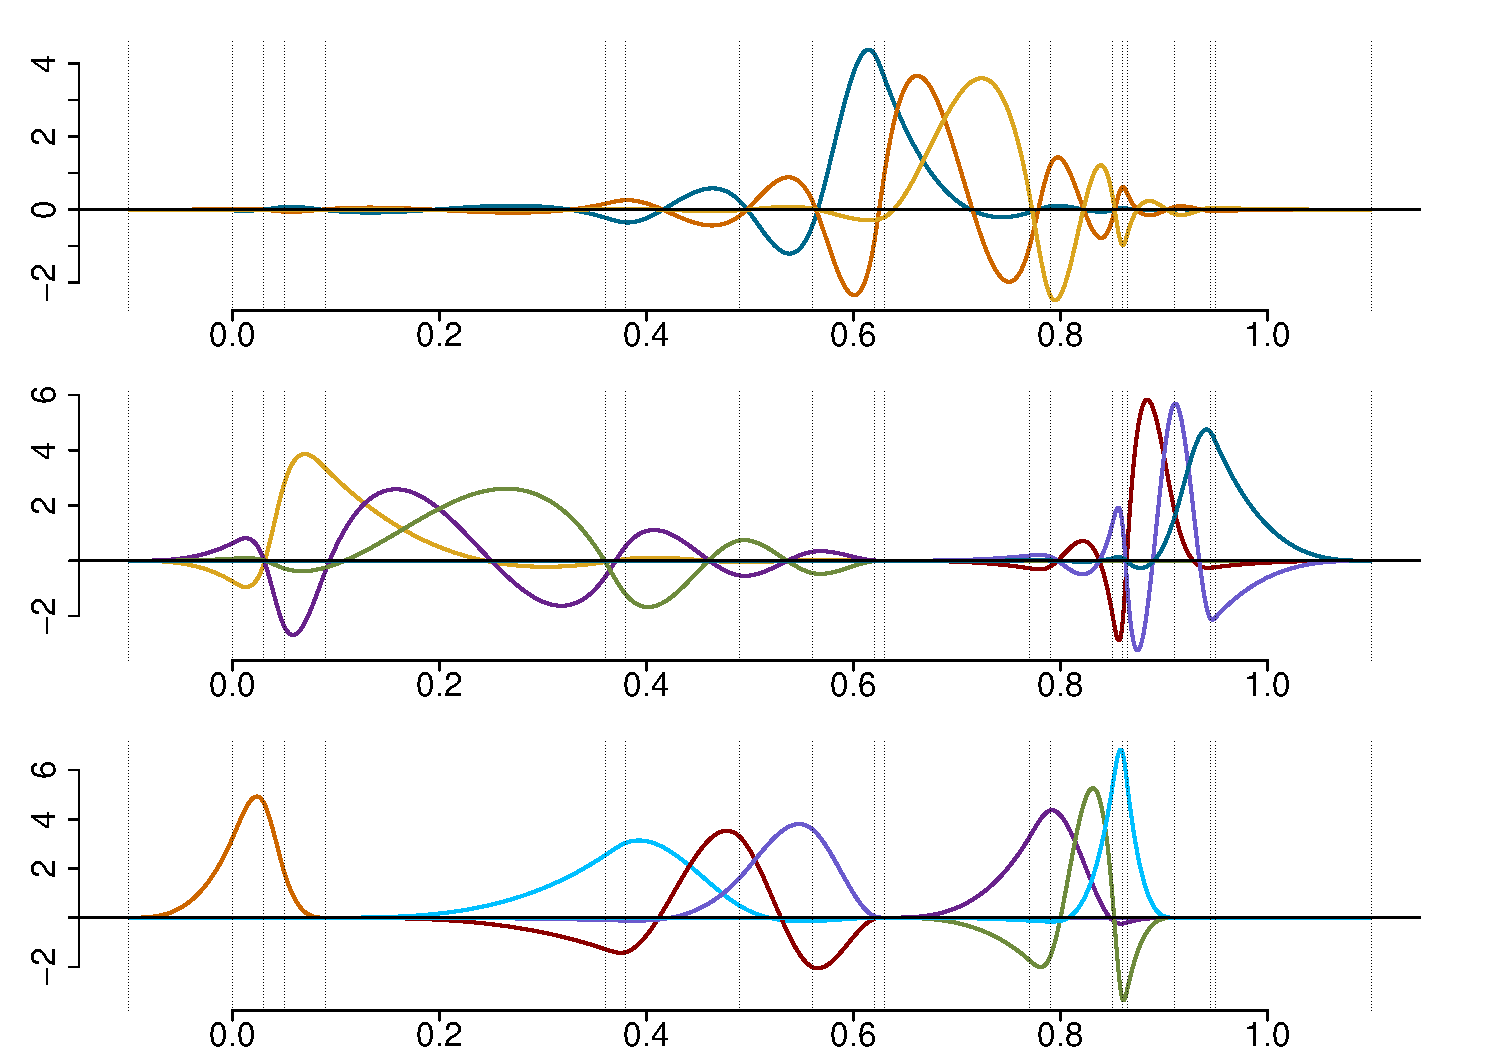
\includegraphics[width=0.59\textwidth]{figures/Fig1LeftSplinet.pdf}\hspace{-2.2cm}
    \raisebox{-1.2cm}{
    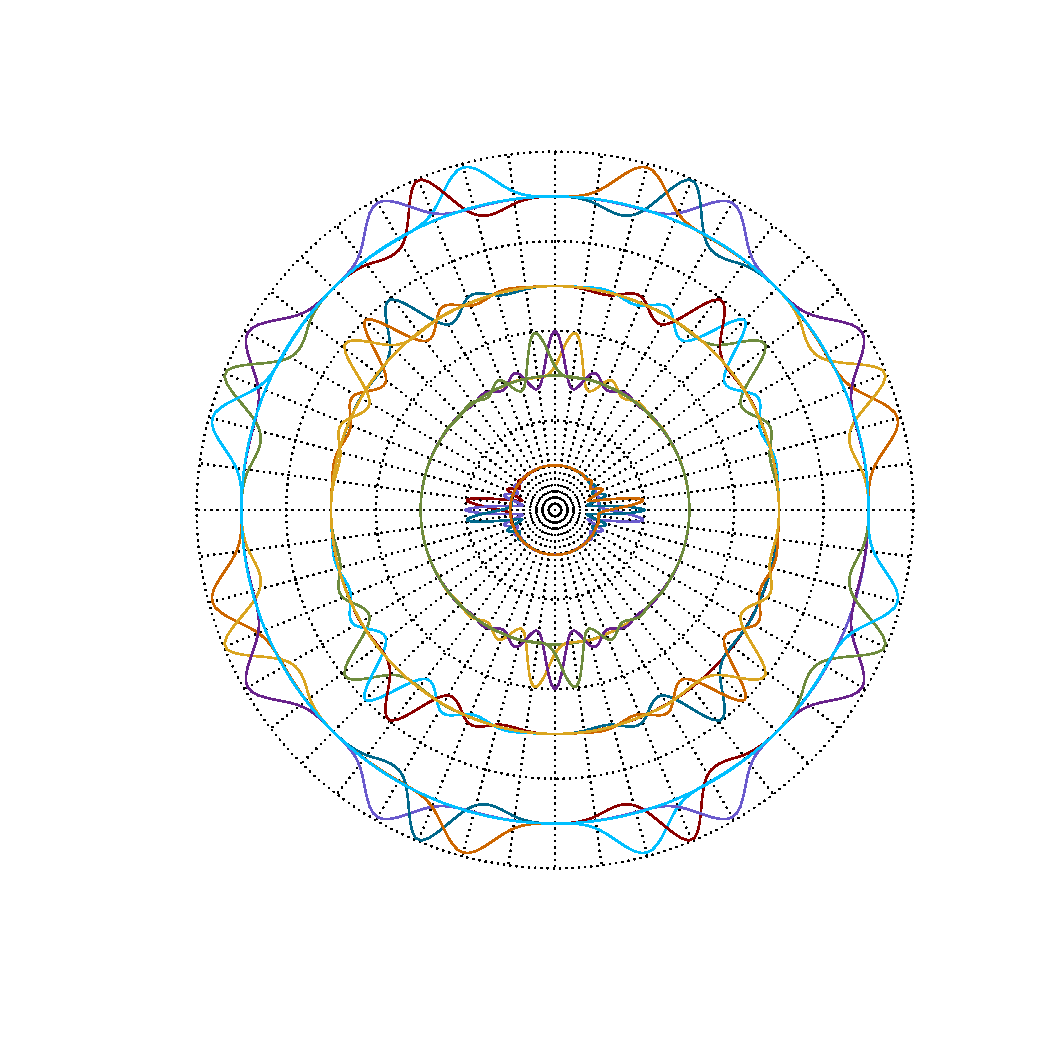
\includegraphics[width=0.59\textwidth]{figures/Fig1RightCircular.pdf}
    } \vspace{-7mm}
    \caption{{\em Splinets} - the orthogonal cubic spline bases presented on dyadic levels: \emph{ (Left)} A splinet made on irregularly spaced knots on an interval, not a complete dyadic case; \emph{ (Right)} Periodic splinet on regularly spaced knots presented on circular dyadic levels, a complete dyadic case of 48 O-splines.}
    \label{fig:splinets}
\end{figure}

% #######
Our goal is to demonstrate that all these features of the \pkg{Splinets} package make it a powerful and effective tool for functional data analysis (FDA). Not only does the package allow for standard methods to be easily implemented, but it also facilitates the exploration of new methodologies that are specific to the choice of splines as functional spaces for analysis.
In fact, the workflow for the classification problem is presented in this paper to demonstrate the capabilities of the \pkg{Splinets} package in various aspects of functional data. The approach is used in a case study of classifying images. 

The organization of the material is as follows. 
The paper starts with the Taylor expansion based functional representation of splines used in the package implementation. 
A discussion of the importance of the spline space selection for the data at hand follows. 
The knot selection is highlighted in this discussion.  
Once a proper spline space is chosen, the projection to the space becomes the main tool in the data analysis as it produces the isometry between functional spaces and  Euclidean spaces.
Thus a presentation of the projection of functions to the space of splines by means of the developed spline bases is discussed next. 
Applications of these basic methods to perform a standard functional analysis through some classical data sets illustrate the methodology. 
The most advanced implementation of the FDA is presented in the final section, where the workflow for the classification problem is elaborated and applied through a case study based on the fashion MNIST data.

\vspace{-.13cm}
\section{ Splinets implementation}
\vspace{-.22cm}
The splines can be represented in a variety of ways. 
In \citet{Qin}, a general matrix representation was proposed that allows for efficient numerical processing of the operations on the splines. 
This was utilized in \citet{Zhou} and  \citet{Redd} to represent and orthogonalize $B$-splines that were implemented in the R-package \pkg{orthogonalsplinebasis} \citep{orthogonalsplinebasis}.
In our approach, we propose to represent a spline in a different way.
Namely, we focus on the values of the derivatives at knots and the support of a spline.  
The goal is to achieve better numerical stability as well as to utilize the discussed efficiency of base splines having support only on a small portion of the considered domain.
In fact, there are three sources of the efficiency and computational stability of the package \pkg{Splinets}:
\begin{description}
\item[Taylor expansion representation] Representing a spline by the matrix of the derivatives at the knots makes use the local Taylor expansion. 
\item[Sparse domains] Implementing partial support sets for splines as well as the spline algebra and calculus that is based on support sets.
\item[Efficient orthogonal bases] Using the dyadic algorithm to orthogonalize the $B$-splines and utilize them in the projection methods. 
\end{description}
The first two features are implemented in the \code{"Splinets"} class, the third one is programmed through an algorithm of intelligent orthogonalization of $B$-splines. 
The efficiency and stability of the representation based on the local Taylor expansions is mathematically justifiable since the matrix of the derivatives at the knots translate directly to the function behaviour locally between knots.  However, we did not explicitly compare computational efficiency with other spline implementations because these features are unique and, to our best knowledge, they are not covered in other packages. Some details are given in what follows, while the topic is more completely elaborated in \citep{podgorski2021}.

%%%%%%%%
\begin{figure}
    \centering
    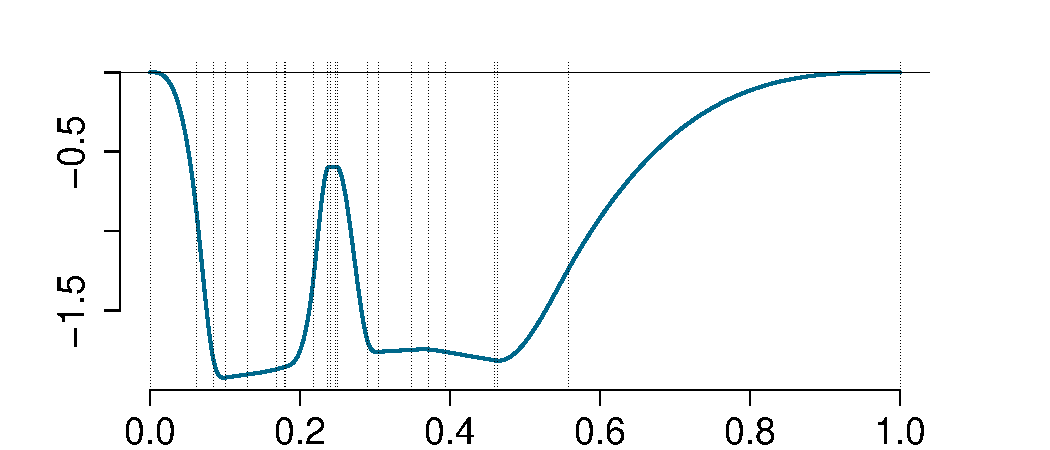
\includegraphics[width=0.52\textwidth]{figures/Fig2LeftTopSpl.pdf}\hspace{-1cm}
     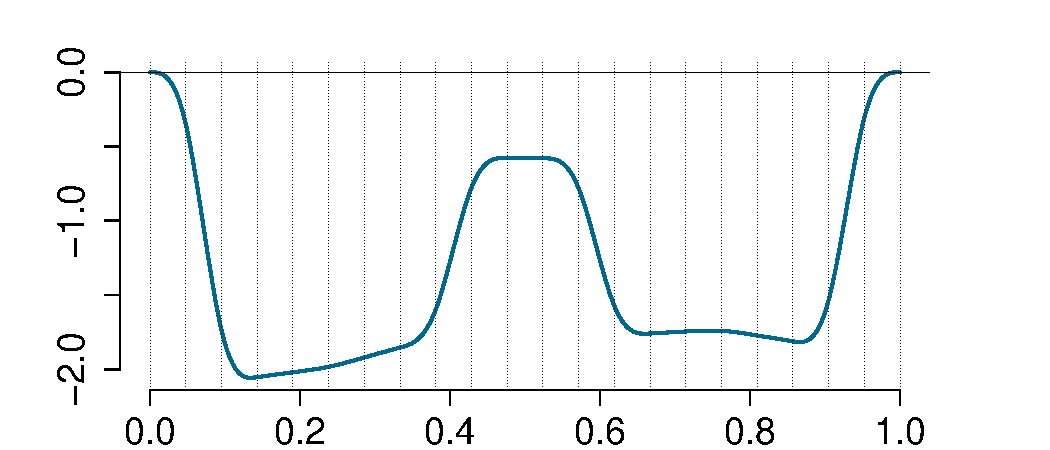
\includegraphics[width=0.52\textwidth]{figures/Fig2RightTopSpl.pdf}\\
      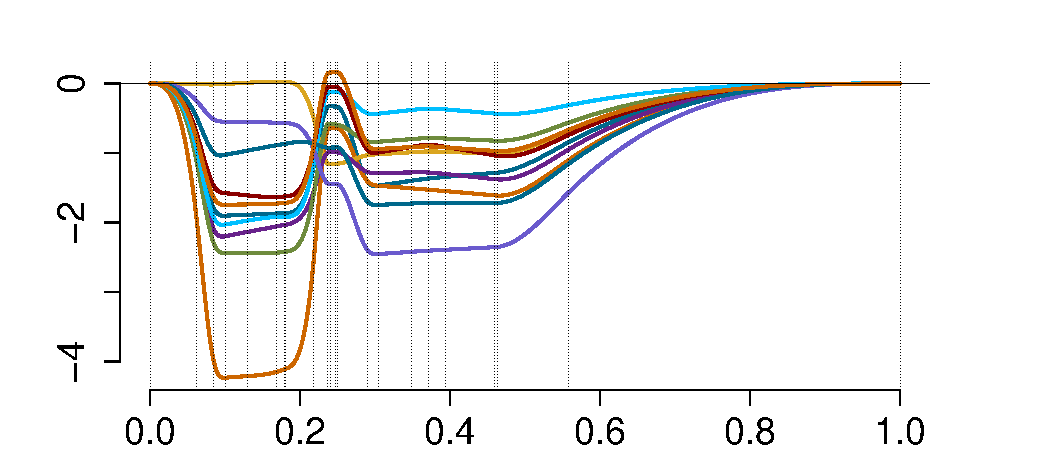
\includegraphics[width=0.52\textwidth]{figures/Fig2LeftBottomSpl.pdf}\hspace{-1cm}
      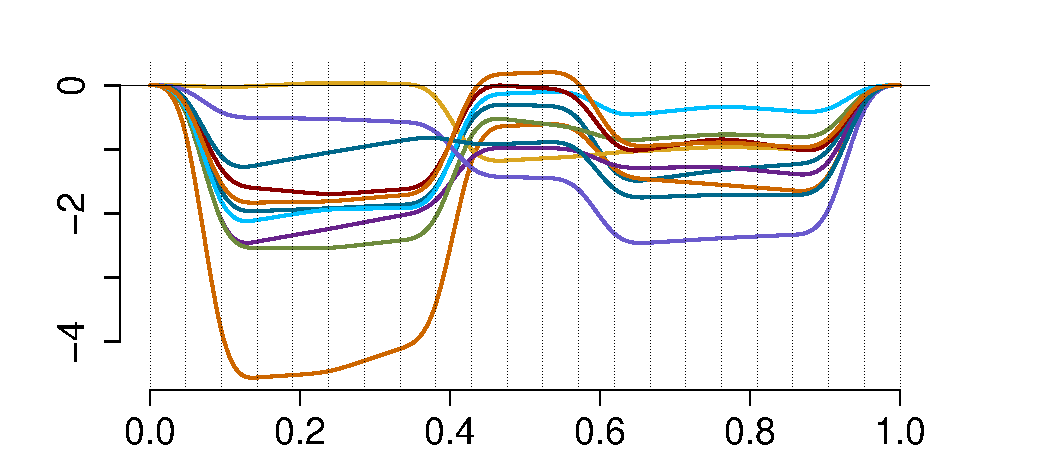
\includegraphics[width=0.52\textwidth]{figures/Fig2RightBottomSpl.pdf}\\
        \caption{Examples of splines for non-equally spaced knots (left) and equally spaced knots (right). In the top graphs, we see individual splines while in the bottom ones random spline samples are generated around the top one by the random spline generator function implemented in the package.  The vertical dashed lines in all figures are placed at the locations of the knots. }
    \label{fig:splinesp}
\end{figure}
%%%%%%%%%

In the following code, a random sample of splines is generated using spline generator implemented in the package.
The result is shown in Figure~\ref{fig:splinesp} and demonstrates that the knot distribution is fundamental in shaping geometry of functional spaces. 
The difference in the nature of the two linear functional spaces  is obvious: in the left graphs we see more focus on the localized variability and detail, the capacity that is lacked in splines in the right-hand side. 
From the analyst point of view, the challenge is to choose a space that matches geometrical characteristics observed in the data. 

\begin{example}
n <- 20  # Number of knots
k <- 3   # Degree of splines
set.seed(10)
xi <- sort(rbeta(n + 2, 2, 5))  # Randomly distributed knots
xi[1] <- 0
xi[n + 1] <- 1 
S <- matrix(rnorm((n + 2) * (k + 1)), ncol = (k + 1))  # Random matrix of derivatives
spl <- construct(xi, k, S)  # A spline object with corrected derivatives matrix
plot(spl)
y <- rspline(spl, 10)  # Random spline generator
plot(y)
xi2 <- seq(0, 1, by = 1 / (n + 1))
spl2 <- construct(xi2, k, S)  # Another spline object
plot(spl2)
y2 <- rspline(spl2, 10)  # Another random sample
plot(y2)
\end{example}

The implementation of a sparse domain is a novel feature not present, as far as we know, in other spline implementations. 
The numerical gains are obvious since we avoid numerical evaluations of operations that are known to be zero. 
In this sense it is similar to the packages for sparse matrices, where zero terms are omitted in the matrix representations. 
The benefits for sparse functional data is illustrated in Figure~\ref{fig:MSSpectrum}-\emph{ (Bottom-right)}.
Additional efficiency in handling functional basis with locality features such as $B$-splines and splinets lies in using the sparse domain feature. 
Indeed, the elements of such bases are non-zero only on small portions of the domain and in evaluating the projection to the spline spaces is significantly faster if the unnecessary operations on zeros are omitted. 

Finally, the package implements, for the first time, an innovative orthogonalization through the numerical efficiency of the dyadic algorithm.
The orthogonal bases obtained in the process are discussed in more detail further in the paper while the algorithm itself and its computational benefits have been demonstrated in \citep{LIU2022}. 


%%%%%%%%%%%%%%%%%%%%
\vspace{-.13cm}
\subsection{Splines with zero-boundary conditions at the endpoints}
\vspace{-.22cm}
Splines are piecewise polynomials of a given {  degree with continuous derivatives up to the degree} (exclusive) at the points they interconnect, which are called \emph{ internal knots}. 
The domain of a spline will be called its \emph{ range} and is assumed in the paper to be a closed finite interval. 
Additional knots called the  \emph{ initial knots} and the \emph{ terminal knots} are located at the beginning and the end of the spline range, respectively.
For a given set of knots, the space of splines is finite-dimensional, with the inner product of the Hilbert space of the square-integrable functions. 


It is worth mentioning two extensions of functional spaces that are handled by the package. 
The first are splines that do not have full support over the entire range of the considered domain. 
This can be of special utility for the sparse functional data, i.e. the functional data that are nonzero only on a small number of locations.
A good example of such data are mass spectra in proteomics or metabolomics analyses. 
The implementation of the \code{"splinet"} object allows specifying a support of functional spline to be only on a union of disjoint intervals inside of the entire range of domain.
The second generalization extends beyond the splines since the \code{Splinets} object can be used to represent any piecewise polynomial function of a given { degree}. All the relevant functions
work properly even if the smoothness at the knots is not preserved. 

Due to the continuity requirements, the behaviour of a spline between two given knots is necessarily affected by the form of polynomials at the neighboring between-knots subintervals. 
Since the between-knots intervals with terminal knots have only one neighboring between-knots interval, the influence of values over other intervals is not the same.   
To mitigate this biased terminal knots effect, it is natural and, as it will be seen, also mathematically elegant to introduce the zero boundary conditions at the terminal knots for all the derivatives except the highest {  degree} one. 
It can be shown that to remove the zero boundary effect, one has to consider splines over the knots obtained through extending by a certain number of knots from both ends of the complete set of knots. 
More specifically, the number of knots that have to be added at each end is equal to the {  degree}  of the splines. 
Often the knots are added by replicating the terminal knots although there are some serious disadvantages of such an approach.

The splines involve knots at which the polynomials smoothly connect. 
A set of such knots is represented as a vector $\boldsymbol \xi$ of $n+2$ ordered values. 
As already mentioned, there are two alternatives, but in a certain sense equivalent, requirements on the behaviour of a spline at the endpoints of its range.
In the first, no boundary conditions are imposed. The main problem in this unrestricted approach is that the polynomials at both ends of the considered range do not `sense' the same restrictions from the neighbors as the polynomial residing further from both endpoints. This is due to the fact that at the endpoints the `neighbors'  are only present from one side.
Another approach, favored in this work, is by putting zero boundary restrictions on the derivatives at the endpoints.
This approach is mathematically equivalent to the first one in a limiting sense, when the $k$ initial knots and the $k$ terminal knots converge to the beginning and the end of the range, respectively.  Moreover and most importantly, the approach is structurally elegant and thus easier to implement.
For all these reasons, it is used in our package.   However, the main object of the package which is \code{"splinets"}.

We impose on a spline and all its derivatives of the {  degree}  smaller than the spline {  degree}  the value of zero at both the endpoints of the range. 
In this case, if we consider knots $\boldsymbol \xi=(\xi_{0},\dots, \xi_{n+1})$
it is important to assume that  $n\ge k$, in order to have enough knots to define at least one non-zero spline with the $2k$ zero-boundary conditions at the endpoints.
Indeed, if $n=k-1$, then we have $k+1$-knots yielding $k$ between knot intervals. 
On each such interval, a spline is equal to a polynomial of {  degree}  $k$.
The dimension of the space of such piecewise polynomial functions is $k(k+1)$. However, at each internal knot, there are $k$ equations to make derivative up to {  degree}  $k$ (excluding) continuous. 
This reduces the initial unrestricted polynomials dimension by $(k-1)k$ dimensions to $2k$, but there are $2k$ equations for the derivatives to be zero at the endpoints.
We conclude that the dimension of the spline space is eventually reduced to zero, meaning that there is only a function trivially equal to zero in this space.
From now on $\mathcal S^{\boldsymbol \xi}_{ k}$ stands for the $n-k+1$ dimensional space of the $k$-smoothed splines with the zero boundary conditions at the terminal knots of in the ordered knots given in vector $\boldsymbol \xi$.
When the dependence on either $k$ or $\boldsymbol \xi$ or both is not important, they will be dropped from the notation. 


The fundamental fact that we use here is that for a given {  degree} , say $k$, and a vector of knot points $\boldsymbol \xi=\left(\xi_0,\dots, \xi_{n+1}\right)$, a spline $S\in \mathcal S$ is uniquely defined by the values of the first $0,\dots, k$ derivatives at the knots.
The values of derivatives at the knots allow for the Taylor expansions at the knots but they cannot be taken arbitrarily due to the smoothness at the knots.   
The matrix of the derivative values is the main component of an object belonging to our main class in the package.
For any spline function $S\in \mathcal S_k^{\boldsymbol \xi}$, we consider $\mathbf s_j=(s_{0j},\dots, s_{n+1j})$ is an $n+2$-dimensional  vector (column) of values of the $j^{\rm th}$-derivative of $S$, $j=0,\dots, k$, at the knots given in vector $\boldsymbol \xi= \left(\xi_0,\dots, \xi_{n+1}\right)$ that, as a general convention for all vectors (also the convention in R,  is treated as a $(n+2)\times 1$ column matrix. 
These columns are kept in a $(n+2)\times (k+1)$ matrix 

%%%%%%
\begin{equation}
\label{eq:spmat}
\mathbf{S} := \left[ \mathbf{s}_0\ \mathbf{s}_1\ \dots\ \mathbf{s}_k \right]
\end{equation}
%%%%%%%



More specifically, the main object \code{"Splinets"} implemented through the S4 system for the OOP in R is defined through \code{setClass} function with the following slots


\begin{example}
representation(knots = "vector", degree = "numeric", equid = "logical", type =
    "character", supp = "list", der = "list", taylor = "matrix", epsilon = "numeric")
\end{example}


\noindent which represents a collection of splines,  all built over the same knots given in \code{knots}, of the {  degree}  $k$ given in {\tt degree}.
Further {\tt supp}  is the list of matrices having row-wise pairs of the endpoints of the intervals, the union of which constitutes the support set of a particular spline,  and the flag {\tt equid} informs about the equally placed knots, for which the computation can be significantly accelerated. 
The matrices of the derivatives at the knots inside the support sets are given in the list {\tt der} of 
 matrices, where an element in the list refers to a particular spline in our collection and the length of the list corresponds to the number of splines in the object.  
Descriptions of other fields are given in the \pkg{Splinets} package but are not crucial for this presentation.

Consequently, the above object corresponds to a spline function $S$ of {  degree}  $k$ over knots in $\boldsymbol \xi=(\xi_0,\dots, \xi_{n+1})$ that is identified as 
$$
S=\left\{k, \boldsymbol \xi,\mathcal I, \mathbf s_0,\mathbf s_1, \dots, \mathbf s_k\right\},
$$
where $\mathcal I=\{(i_1, i_1+m_1+1), \dots,(i_ N,i_N+m_N+1) \}$ is a sequence of ordered pairs of indexes in $\{1,\dots,n+2\}$ representing the intervals, the union of which is the support of a spline, i.e. the minimal closed set outside  of which spline vanishes.

% ##########
\vspace{-.13cm}
\section{Spline spaces for FDA}
\vspace{-.22cm}
% ##########
One of the fundamental aspects of functional data analysis is the decision in which functional space the functional data (FD) in hand are assumed to be located. 
FD are not observed as continuous objects, but high-frequency sampling and mathematical efficiency enable us to
see these data as samples of curves, surfaces, or anything else varying over a continuum. The fundamental step in FDA
is to convert this discrete recorded data to a truly functional form, which allows each function to be evaluated at any
value of its continuous argument. In order to utilize the topology of such data for dimension reduction, one must perform
data conversion. Typically, one represents a functional object as a linear combination of a suitably chosen basis functions. 
For this purpose, one of the standard bases such as trigonometric, wavelet, or polynomial is typically chosen. 
Then the efficiency is accomplished by using smoothing through regression or roughness penalty for estimating the coefficients of the basis expansions. 

One can argue that the spline bases with their flexibility that comes from the knot selection and the {   degree of splines} make these spaces ideal for 
 efficiency in retrieving the functional
structure of a studied model, see also \citep{basna2022data}.
 The splines involve knots at which the polynomials smoothly connect. 
A set of such knots is represented as a vector $\boldsymbol \xi$ of $n+2$ ordered values. 
In this work, we consider the zero-boundary version of splines by putting zero boundary restrictions on the derivatives at the endpoints.
This approach is mathematically equivalent to the first one in a limiting sense, when the $k$ initial knots and the $k$ terminal knots converge to the beginning and the end of the range, respectively.  Moreover and most importantly, the approach is structurally elegant and thus easier to implement.
For all these reasons, it is used in our package.   
The central object of the package is \code{"splinets"}, which represents a sequence of splines and holds it in the object by coefficients of the Taylor expansion of the function at the knots, which uniquely defines a spline using a matrix of derivatives at the knots. 



The fundamental feature of the package and of the approach to FDA are the efficient orthogonal bases, the so-called splinets, which allow for a very efficient data representation. 
These bases that were introduced in \citep{LIU2022} are discussed next. 


% ##########
\vspace{-.13cm}
\subsection{Splinets -- orthonormal bases of splines}
\vspace{-.22cm}
%%%%%%
The direct approach to building splines requires a lot of care and often can be cumbersome. 
A more efficient approach is through functional bases of splines. 
There are many possible choices of such bases but the most popular are the $B$-splines. 
Despite having many advantages, the $B$-splines do not constitute an orthogonal basis, which is a computational problem as the projection to the non-orthogonal bases adds to the numerical complexity. 
This challenge occurs in implementing the orthogonal projection operator discussed in the next subsection. 
On the other hand, using the orthogonality of the splinet allows an efficient representation of the data also in $B$-splines because the matrix conversion from one basis to another is sparse.
The main feature of the package is to implement an optimal orthogonalization of the $B$-splines into the orthogonal bases called \emph{splinets} introduced in \cite{LIU2022}. 
The graphical presentation of the spline basis visually benefits from organizing them in the form of a dyadic net that corresponds to the dyadic orthogonalization procedure applied to the $B$-splines, the technical definition of the dyadic net and further details can be found in \cite{LIU2022}. 
However, this dyadic net representation is used mostly for the visualization and one can equally use the sequential representation if preferred.
The package facilitates simple switching between the two representations. 
In Figure~\ref{fig:Orth}, one can see $B$-spline basis in the left graphs and the corresponding  splinet in the right. 
In the top graphs, we use the sequential graphical presentation and in the bottom ones the dyadic form that allows for a better inspection of the basis functions. 


The orthonormalized bases implemented in this package are obtained by one of the following three orthogonalization procedures applied to $B$-splines. 
The first one is simply the Gram-Schmidt orthogonalization performed on the $B$-splines ordered by their locations, the second one is a symmetric (with respect to the knot locations) version of the Gram-Schmidt, and, finally, the dyadic orthogonalization into a {\em splinet} which is our preferred method. 
We will not discuss the first two orthonormalization methods as they have been included in the package mostly because of historical reasons. 
In the object representation of collections of splines, i.e. in the \code{"Splinets"} class, the field \code{type} specifies which of the orthonormal basis one deals with. 
The function  \code{splinet()} is generating the proper basis as illustrated the code that creates the $B$-splines, the corresponding splinet and the graphical illustration shown in Figure~\ref{fig:Orth}

\begin{example}
k <- 3        # Degree of splines
N <- 5        # Number of layers
n <- k * 2^N - 1  # Number of knots
set.seed(2)
xi <- cumsum(runif(n + 2, min = 0.2))  # Random knots
so <- splinet(xi, k)  # Evaluation of the B-splines and the splinet
plot(so$bs, type = "dyadic")  # B-splines on the dyadic net
plot(so$os)                   # Splinet on the dyadic net
\end{example}


One can observe that \code{splinet()} is returning a list of two \code{Splinets} objects, \code{so\$bs} and \code{so\$os} build over the ordered knots {\tt xi}.
The first object represents the basis of the standard cubic $B$-splines and is thus not orthogonal. 
The second one represents the recommended orthonormal basis, which is referred to as a cubic splinet. 
In Figure~\ref{fig:Orth}~\emph{(Right)}, one can see the splinet obtained from the $B$-splines given in the right-hand side.

%%%%%%

\begin{figure}[t!]
\centering
\raisebox{-0.6cm}{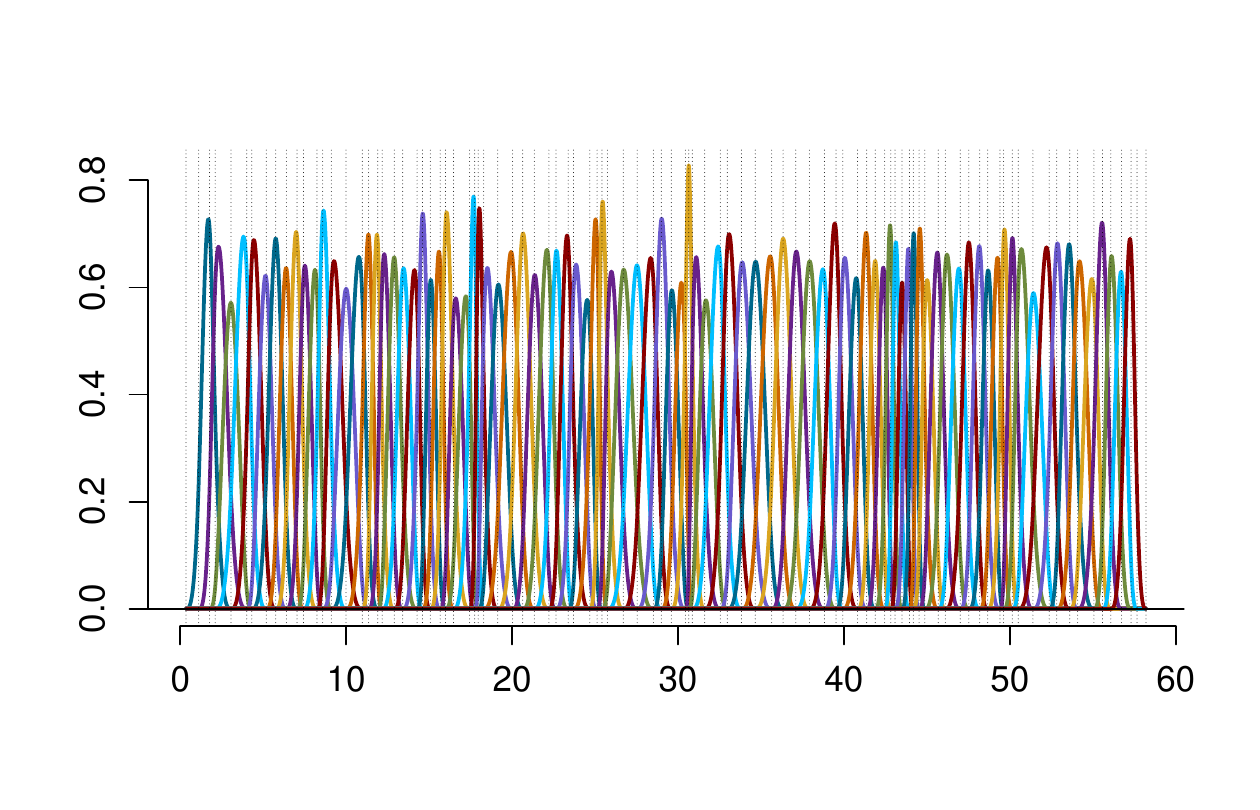
\includegraphics[width=0.495\textwidth]{figures/Fig3LeftTopSplnt.pdf}}
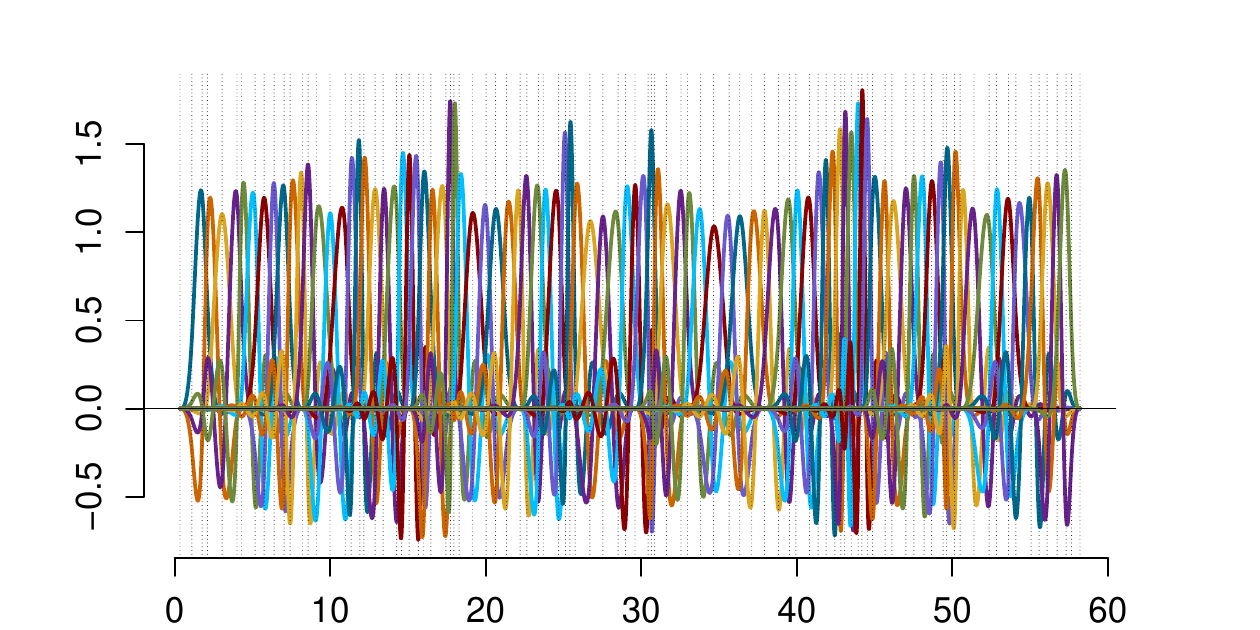
\includegraphics[width=0.495\textwidth]{figures/Fig3RightTopSplnt.pdf} \vspace{-6mm}\\
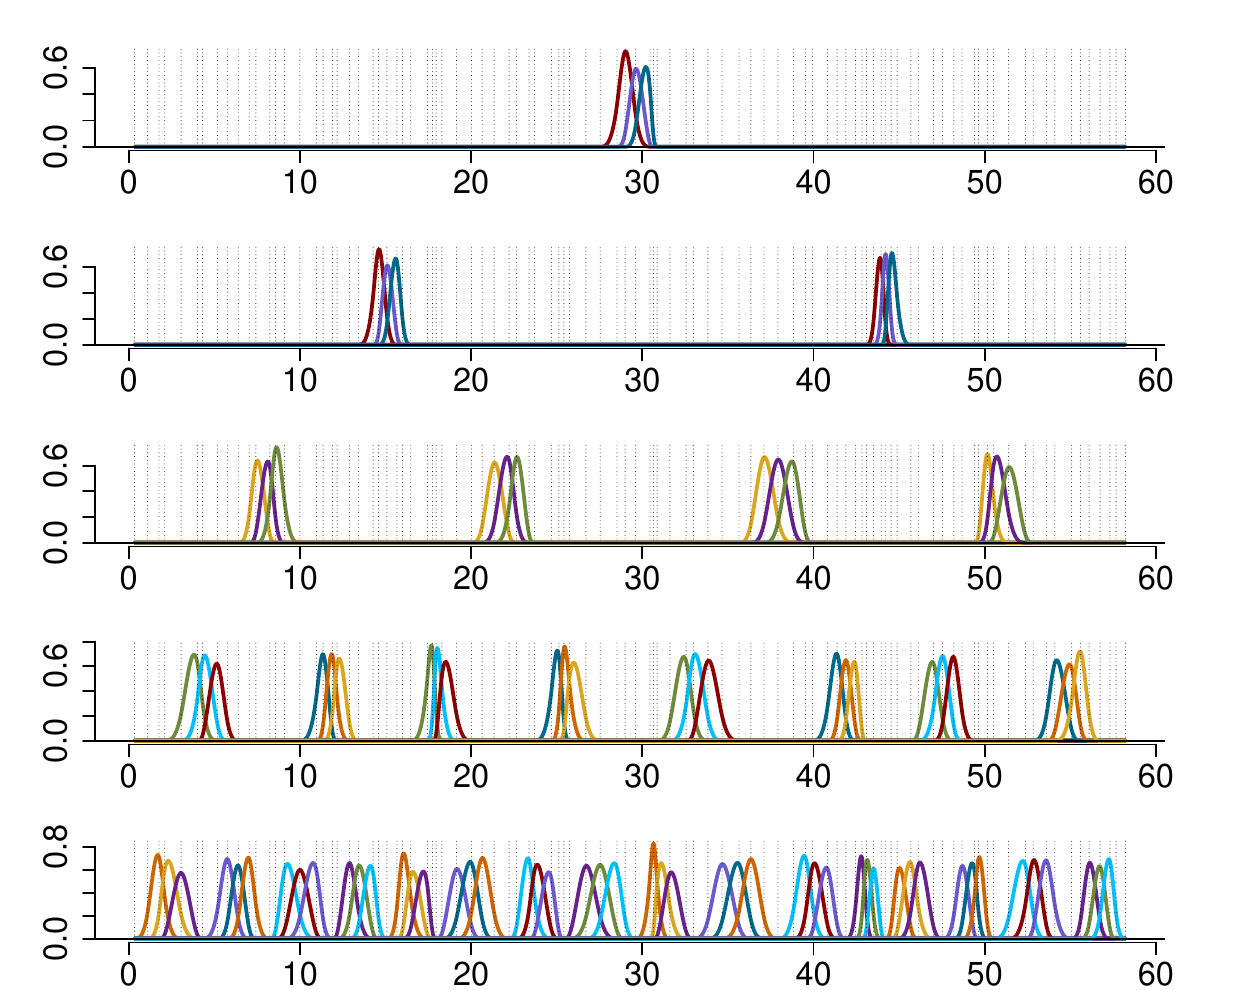
\includegraphics[width=0.495\textwidth]{figures/Fig3LeftBottomSplnt.pdf} 
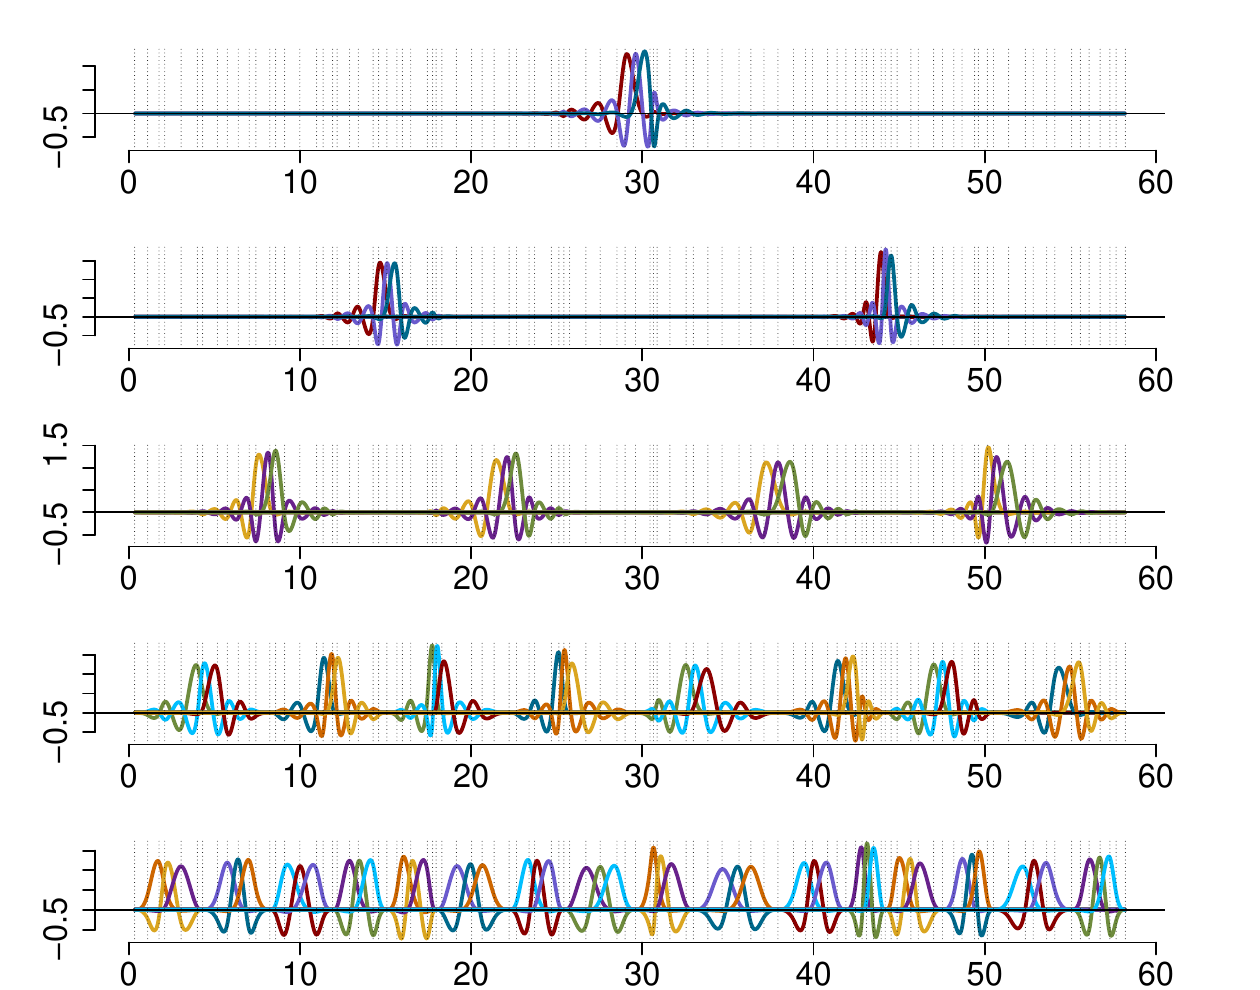
\includegraphics[width=0.495\textwidth]{figures/Fig3RightBottomSplnt.pdf}  
    \caption{\footnotesize  Cubic spline bases presented graphically in the sequential form (top) and on the dyadic net (bottom). The case of $n=k2^N-1=95$, $k=3$, $N=5$ which is the number of layers in the dyadic structure seen in the figures. \emph{(Left)}: The $B$-spline basis; 
  \emph{(Right)}: The corresponding splinet.}
  \label{fig:Orth}
\end{figure}

%%%%%%

\vspace{-.13cm}
\subsection{Projection to space of splines}
\vspace{-0.2cm}
Splines with a given knot selection constitute finite-dimensional subspaces of the Hilbert space of square-integrable functions. 
Thus, any such function can be projected orthogonally into the space of splines defined by a particular set of knots. 
Functional data analysis typically begins by projecting discretized data onto such a finite-dimensional functional space, making the projection a fundamental operation in statistical analysis. 
Projections can also serve as a smoothing step, and various methods are available for this purpose. 

In the package, orthogonal projection is implemented via the function \code{project()}. 
Since functional data may be represented in different ways, the actual projection depends on the input format, especially how the inner product with a spline is evaluated numerically. 
The input to \code{project()} can either be \code{Splinets} objects or a matrix with two columns representing the arguments and values of discretized functional data.

The output of the function is a list with three components:
\begin{description}
\item[\code{projsp\$coeff}] A matrix of coefficients for the decomposition in the selected basis;
\item[\code{projsp\$basis}] The \code{Splinets} object representing the selected basis;
\item[\code{projsp\$sp}] The \code{Splinets} object representing the projection of the input data.
\end{description}

Additional details—such as the knots, degree, and basis type—can be retrieved from \code{projsp\$basis}. 
Many algebraic operations on splines are more efficiently performed on the coefficient matrix rather than directly on the \code{Splinets} objects. 
The matrix \code{projsp\$coeff} can be used for such tasks, while linear combinations of \code{projsp\$basis} yield the corresponding functional forms.

To highlight the simplicity and utility of \pkg{Splinets}, we apply it to mass spectrometry data in a basic numerical example. 
This class of data is particularly suited to the package due to its sparse nature and the computational advantages of localized spline bases. 
We consider a low-resolution SELDI-TOF mass spectrum available from the National Cancer Institute, Center for Cancer Research, Clinical Proteomics Program (\url{https://home.ccr.cancer.gov/ncifdaproteomics/ppatterns.asp}, accessed 2024-05-26). 
For related work using such data, see \citet{Petricoin:2002aa}.

%%%
\begin{figure}[t!]
    \centering
    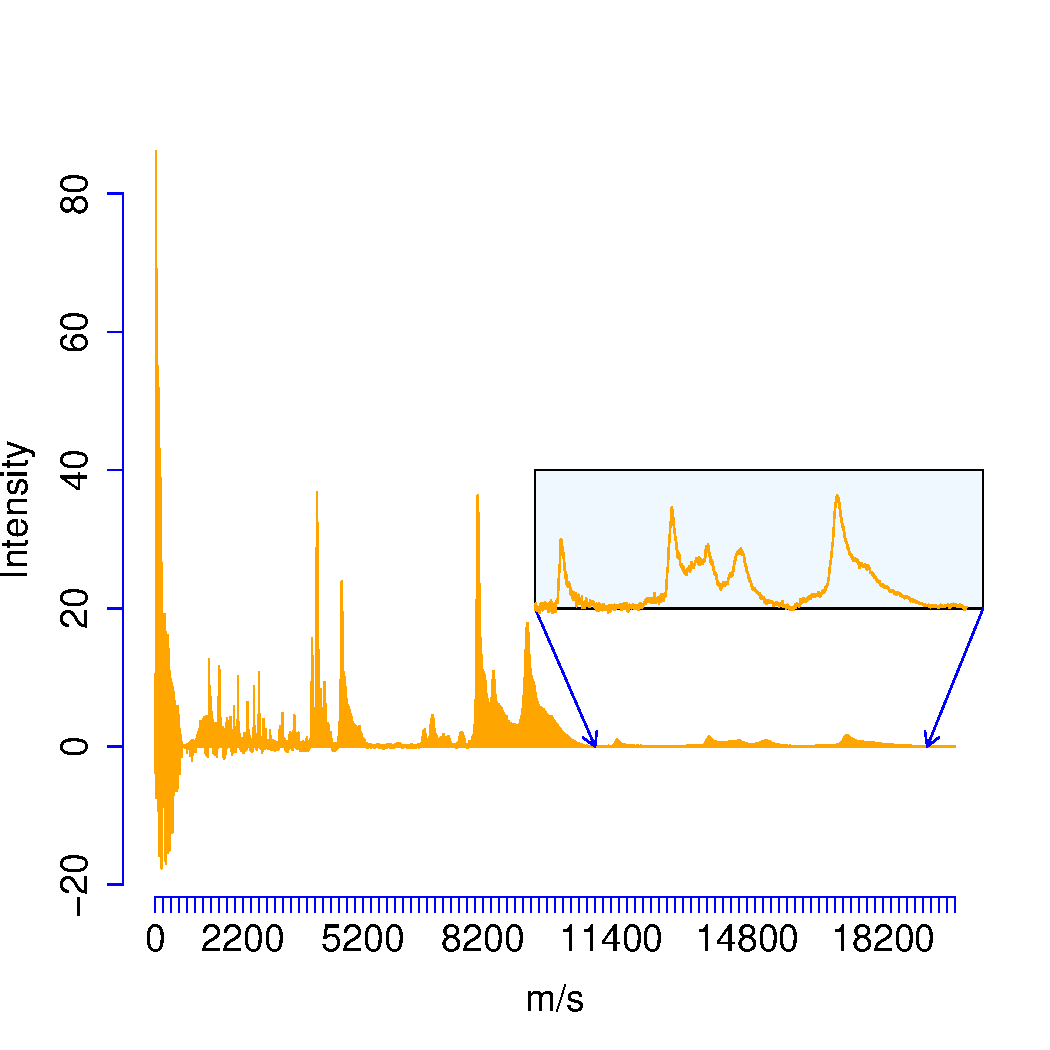
\includegraphics[width=0.49\textwidth]{figures/Fig4LeftTopMS.pdf} 
    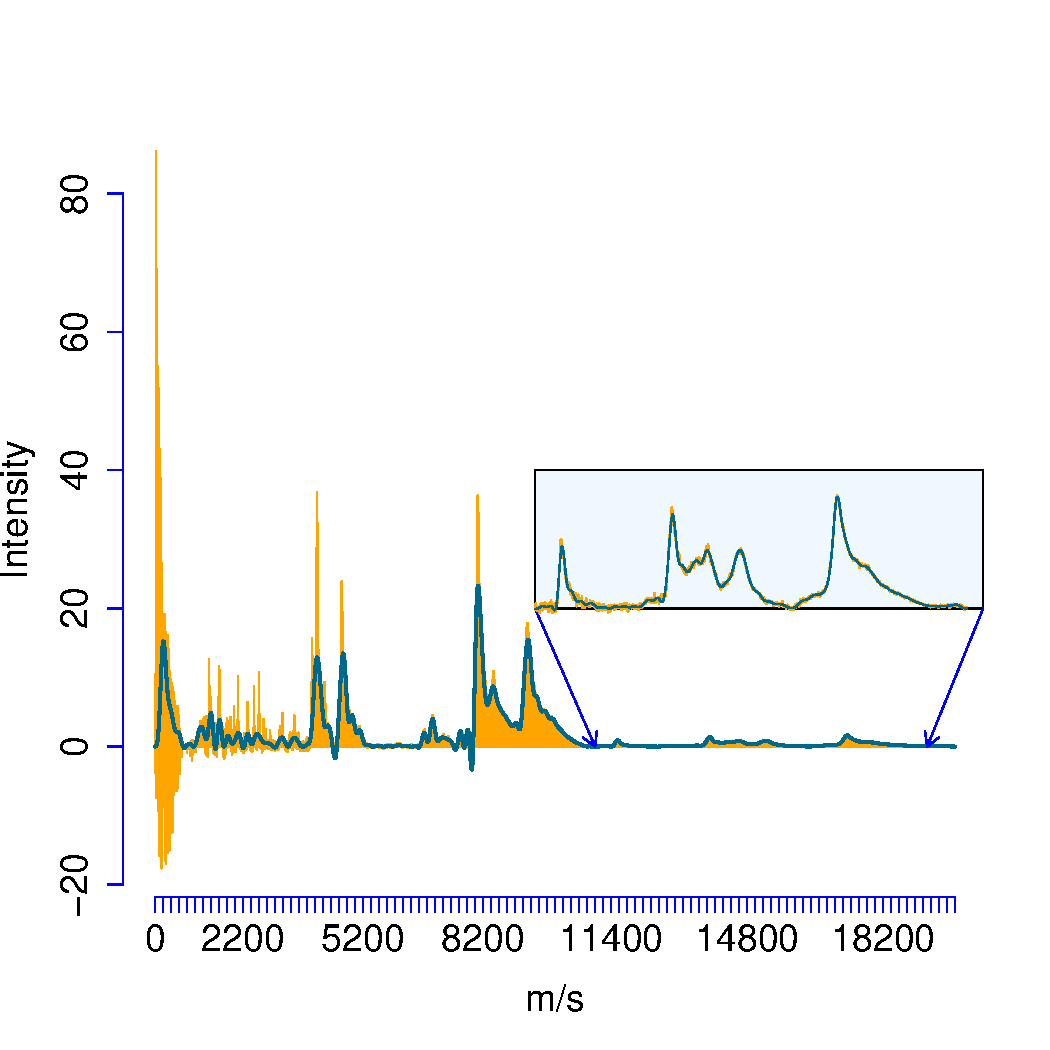
\includegraphics[width=0.49\textwidth]{figures/Fig4RightTopMS.pdf} \vspace{-1.2cm}\\
    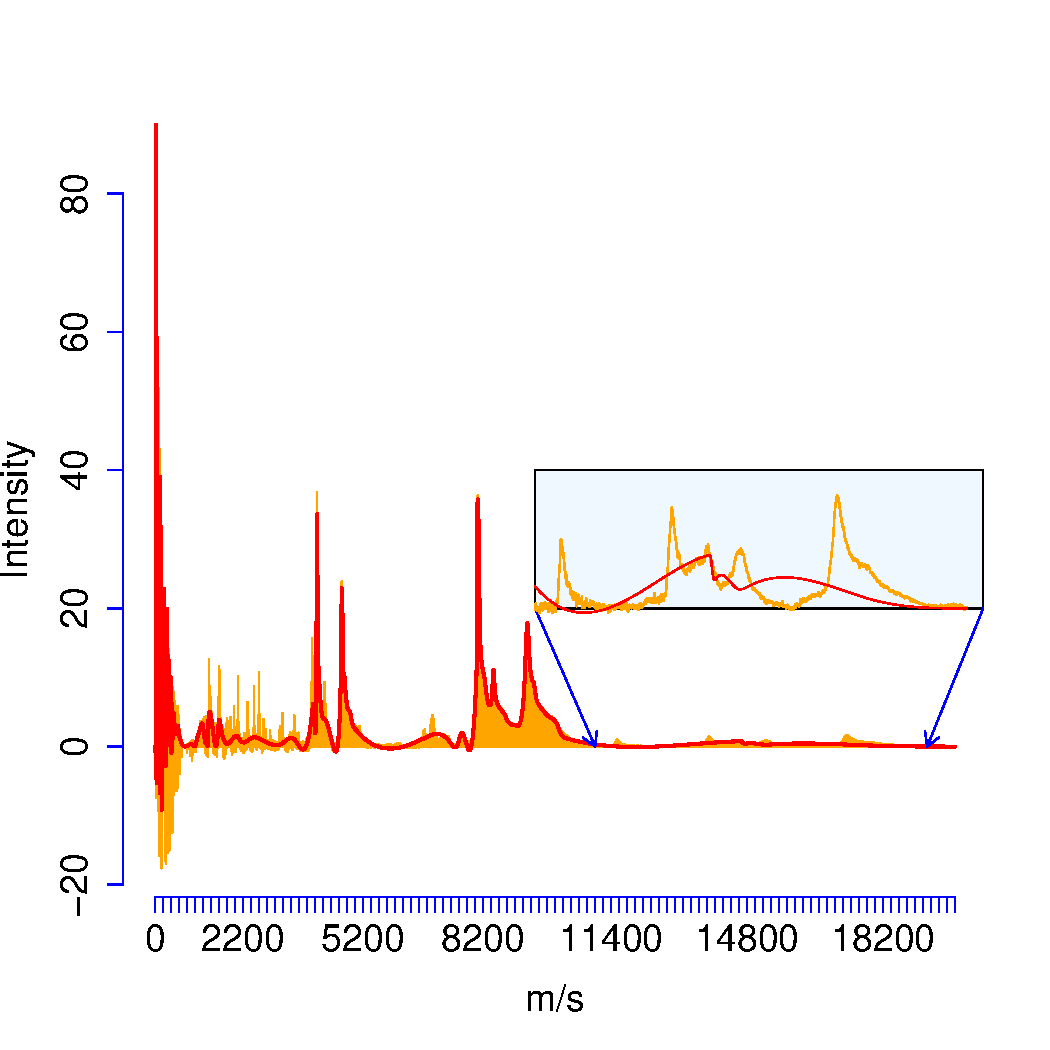
\includegraphics[width=0.49\textwidth]{figures/Fig4LeftBottomMS.pdf} 
    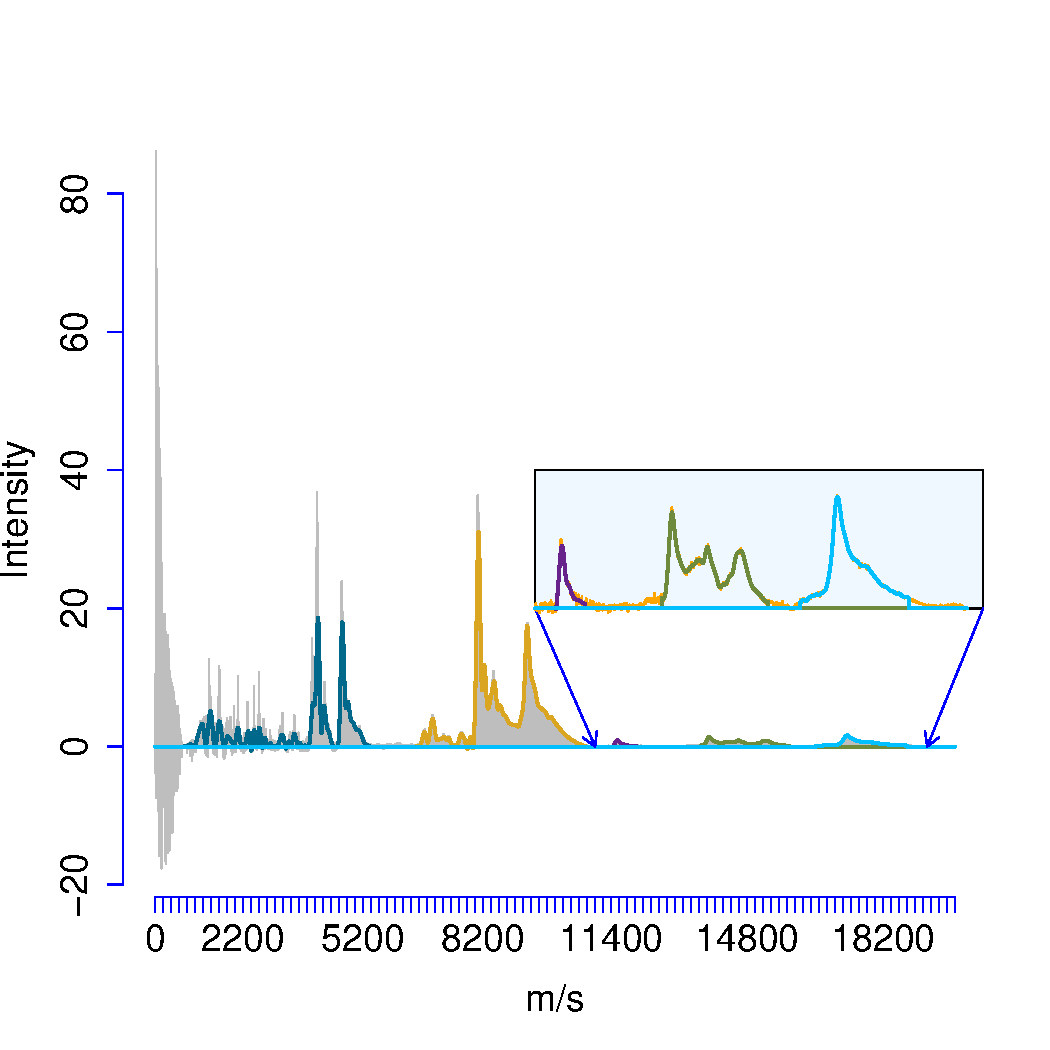
\includegraphics[width=0.49\textwidth]{figures/Fig4RightBottomMS.pdf} \vspace{-3mm}
        \caption{\footnotesize  An ovarian cancer tissue low-resolution SELDI-TOF mass spectrum (in orange) and its various representations as \emph{Splinet}-objects in approximately 200 dimensional spline spaces: \emph{(Top-Left)} The original sample (orange) consisting of 15154 values; \emph{(Top-Right)} The projection (navy-blue) to the spline space spanned on 200 equally spaced knots; \emph{(Bottom-Left)} The projection (red) to the spline space spanned on 200 non-equally spaced knots with their locations chosen by the spectrum; \emph{(Bottom-Right)} The projection to the splines with a sparse domain obtained by specifying five importance regions, with the graph above each of the five support intervals drawn by a different color.\vspace{-5mm}}
    \label{fig:MSSpectrum}
\end{figure}
%%%


In Figure~\ref{fig:MSSpectrum}, we present flexible ways of representing the original signal by different \pkg{Splinets} objects. From these simple illustrations, one can see dramatic reduction from the original 15154 dimension of the data to three different 200 dimensional spline representations that emphasize different and subtle feature in the data. 
The focus here is on the efficiency and flexibility by showing that 200 dimensional spline spaced can be molded toward particular features of interest.
We conclude that even without any in-depth FDA, one can get a significant simplification and dimension reduction of the data at the data representation level. 
In this work, we show that also advanced FDA can be easily implemented with the help of the package.


The simplicity of using the \pkg{Splinets} package can be seen again in the following code examples. If the \code{Ovarian} data and the \pkg{Splinets} package are loaded, then the projection to splines with equally spaced knots is simply obtained by

\begin{example}
xi1 <- seq(min(Ovarian\$ms), max(Ovarian\$ms), length.out = 200) # Equally spaced knots 
so1 <- splinet(xi1)                                       # Orthogonal basis of splines
OvSpl1 <- project(as.matrix(Ovarian), basis = so1\$os)        # Projection to the basis
\end{example}
\noindent the projection to the data driven choice of knots by

\begin{example}
wghts <- abs(Ovarian\$Intensity)/sum(abs(Ovarian\$Intensity))  # Knot selection weights
xi2 <- sort(sample(Ovarian\$ms, 200, prob = wghts))            # Random knots
so2 <- splinet(xi2)                                        # Orthogonal basis of splines
OvSpl2 <- project(as.matrix(Ovarian), basis = so2\$os)         # Projection to the basis
\end{example}


\noindent and the representation by a spline \code{OvSpl4} with a sparse domain with five interval components, which requires a bit more coding, is presented only on the graphs while the code is available in the package vignette at \url{https://ranibasna.github.io/R-Splinets/articles/MassSpectrometry.html}.

\noindent The omission of the first group of knots from the support is due to its noisy character that typically is not of interest in the mass-spectrometry data analysis.

\noindent The package provides a plot method for \code{Splinet} objects, so all the plots from Figure~\ref{fig:MSSpectrum} can be simply obtained through:
\begin{example}
plot(Ovarian\$ms, Ovarian\$Intensity, type = "h")
lines(OvSpl1\$sp)
lines(OvSpl2\$sp) 
lines(OvSpl3)
\end{example}

 The complete code, which facilitates experimentation, demonstrates data analysis, performs the classification procedure, and allows for the recreation of all figures and results, is available as R files with comments. The R code is provided in the supplementary materials on the {GitHub page} \url{https://github.com/ranibasna/R-Splinets} with the accompanied {package site} \url{https://ranibasna.github.io/R-Splinets/index.html}.

 In the discussion of the projection to the spline spaces, we discuss four different types of the projection: embedding, basis decomposition, spline projection, and discretized data projection. 
This functionality is illustrated by a numerically simulated example.

\noindent\emph{Embedding a spline into higher-dimensional spaces of splines.} 
The first function that we discuss is an embedding rather than a projection. 
One of the most interesting aspects of spline spaces is their agility attributed to different choices of the knots.
Yet, when employing splines for functional data analysis, the focus is typically on splines with a fixed, often equally spaced, set of knots, rather than exploring this adaptability.
In the proposed package, we provide tools to thoroughly explore the properties of splines under various knot choices. 
Any spline remains a spline of the same \emph{degree} when considered on a set of knots larger than the original.
However, this changes the \code{Splinets} object representation of the refined spline. 
It is thus important to have a function that embeds a given spline into a larger space of splines defined on a refined set of knots. 
In the package, the function \code{refine()} allows splines from smaller spaces to be conveniently represented in larger, more refined spaces.

\noindent\emph{Basis decomposition.} The simplest projection obtained through \code{project()} is also not, strictly speaking, a projection but rather a decomposition of a \code{Splinets} object into coefficients in the given basis. 
If \code{sp} is a \code{Splinets} object, then the code

\begin{example}
bdsp <- project(sp)
bdsp2 <- project(sp, type = "bs")
\end{example}

\noindent have as its main output the matrices of coefficients $a_{ji}$, such that the $j^{\text{th}}$ input-spline $S_j$ that is in the input \code{sp} has the form
\[
S_j = \sum_{i=1}^{n-k+1} a_{ji} B_{i},
\]
where $j$ indexes the input splines, $n$ is the number of the internal knots (the knots not including the two endpoints of the domain), $k$ is the degree of splines, and $B_{i}$'s are the elements of the selected basis of splines controlled by the input \code{type}, so in the above example it is either the splinet (\code{bdsp}) or the $B$-spline basis (\code{bdsp2}). 
The bases are built on the same knots as the input spline.

\noindent\emph{Projecting splines.}
The projection of \code{Splinets}-objects over a given set of knots to the space of splines over a different set of knots is obtained through the orthogonal projection:
\begin{example}
bdsp <- project(sp, knots)
bdsp2 <- project(sp, knots, type = "bs")
\end{example}

\noindent
The results are represented in the spline space built over \code{knots}, and thus the \code{Splinets}-object in the output representing the projection spline satisfies \code{bdsp\$bs@knots = knots}. 
Namely, if $S_j$ is the input \code{Splinets}-object, then the output is denoted as $\mathbf{P} S_j$, where $\mathbf{P}$ is the orthogonal projection to the space spanned by the spline basis constructed from the second set of knots:
\begin{equation}\label{projection}
\mathbf{P} S_j = \sum_{i=1}^{n - k + 1} a_{ji} B_i, \quad (S_j - \mathbf{P} S_j) \perp \mathbf{P} S_j,
\end{equation}
where $B_i$ are elements of the specified spline basis, and \code{knots} can differ from \code{sp@knots}.

This is an extension of the previous case since the output functions may belong to a different space than the input functions.  
The output is obtained by embedding both the input splines and the projection space to the space of splines that contains both built over the union of the two sets of knots.

\noindent\emph{Projecting discretized functional data.}
The function \code{project()} works also when the input is not a spline object but discretized functional data.
This is the most important projection for FDA. 
In this case, the input is a matrix having in the first column a set of arguments and in the remaining ones the corresponding values of a sample of functional data. 
The input data are treated as piecewise constant functions with the value over two subsequent arguments equal to the value in the input corresponding
to the left-hand side argument.
In this way, the discretized data are viewed as functions, and their inner products with any spline are well defined. 
Consequently, the projection $\mathbf P S_j$ of the functional data in $S_j$ satisfies (\ref{projection}), if $S_j$ represents the discretized datum as a  piece-wise constant function. 

\vspace{-.13cm}
\subsection{Spectral decomposition of the wine dataset -- an example of FDA}\vspace{-.22cm}

We use the \code{Splinets} R package to perform Functional Principal Component Analysis (FPCA) on a wine dataset that includes 124 samples, with absorbance measurements taken across 256 wave numbers in the mid-infrared spectrum (4000 to 400 cm$^{-1}$). These spectral characteristics capture key aspects of the chemical composition of the wines, such as alcohol content and sugar content. The wine dataset is provided by Professor Marc Meurens of the Université Catholique de Louvain \citep{benoudjit2004}. To initiate the analysis, we project the discrete data onto orthogonal spline bases using the \code{project()} function. This step transforms the discrete absorbance values into a functional representation utilizing a selected set of knots.

\begin{example}
WineProj <- project(WineData, knots) # Project wine data into the spline space.
\end{example}

It is assumed here that the \code{WineData} data object is processed. The preprocessing steps of the data can be found at the \emph{wine data example package vignette page} \url{https://ranibasna.github.io/R-Splinets/articles/FunctionalPrincipalValueDecomposition.html}.

The use of an orthogonalized functional basis provides significant computational advantages, reducing the complexity of performing FPCA on the functional data. By projecting the data onto an orthogonal basis, we benefit from simplifying the process of finding the functional principal components. This is because, in an orthogonal basis, the functional principal components can be efficiently derived by performing PCA on the projection coefficients.

Without orthogonality of the basis (like in the B-spline case), doing so would not be correct. The functional principal components can be computed as a linear combination of the eigenvectors and the spline basis.

\begin{example}
Sigma <- cov(WineProj\$coeff)    # Covariance matrix of the projection coefficients
Spect <- eigen(Sigma)            # Spectral decomposition of the covariance
EigenSp <- lincomb(WineProj\$basis, t(Spect\$vec))  # Functional eigenfunctions
\end{example}

\begin{figure}[t]
    \centering
    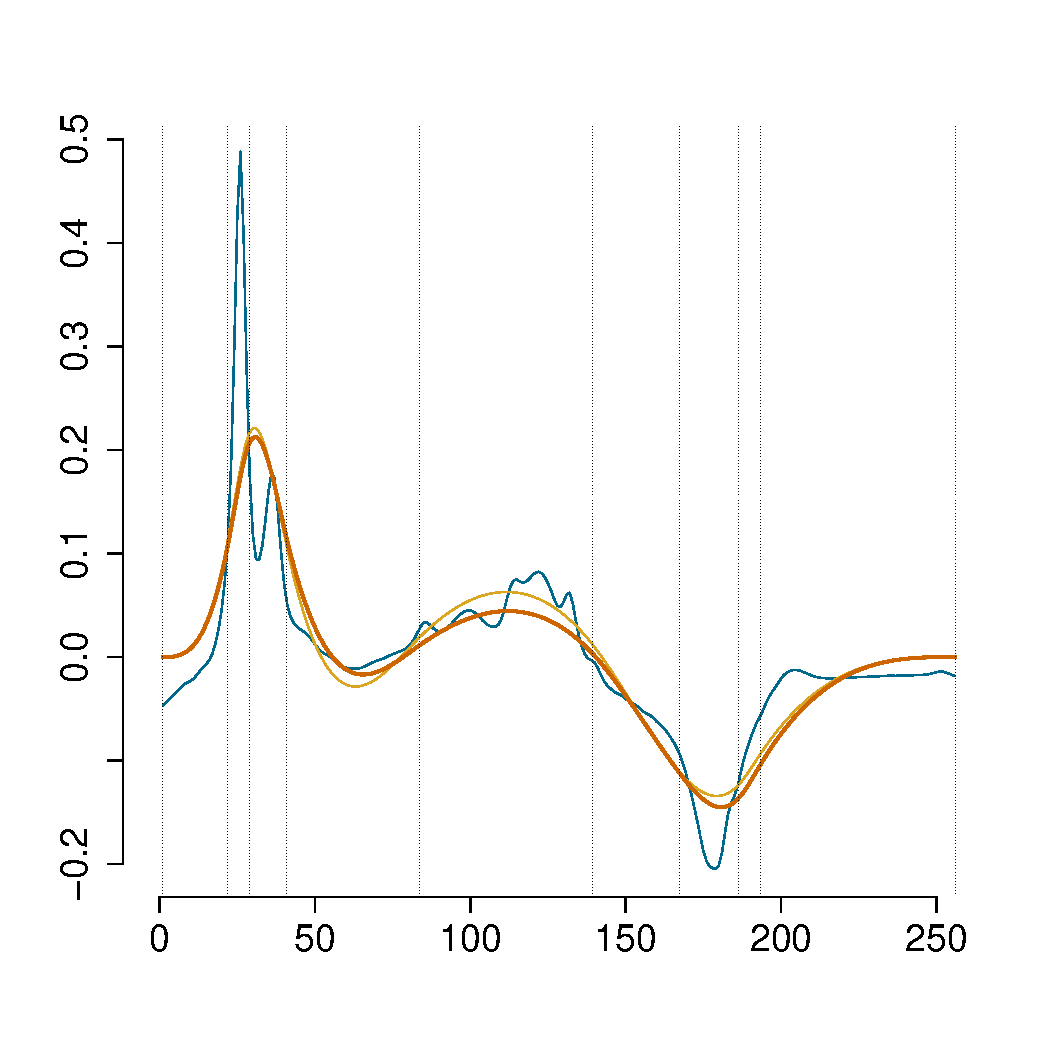
\includegraphics[width=0.5\linewidth]{figures/Fig5LeftFhatWine.pdf}\hspace{-2mm}
    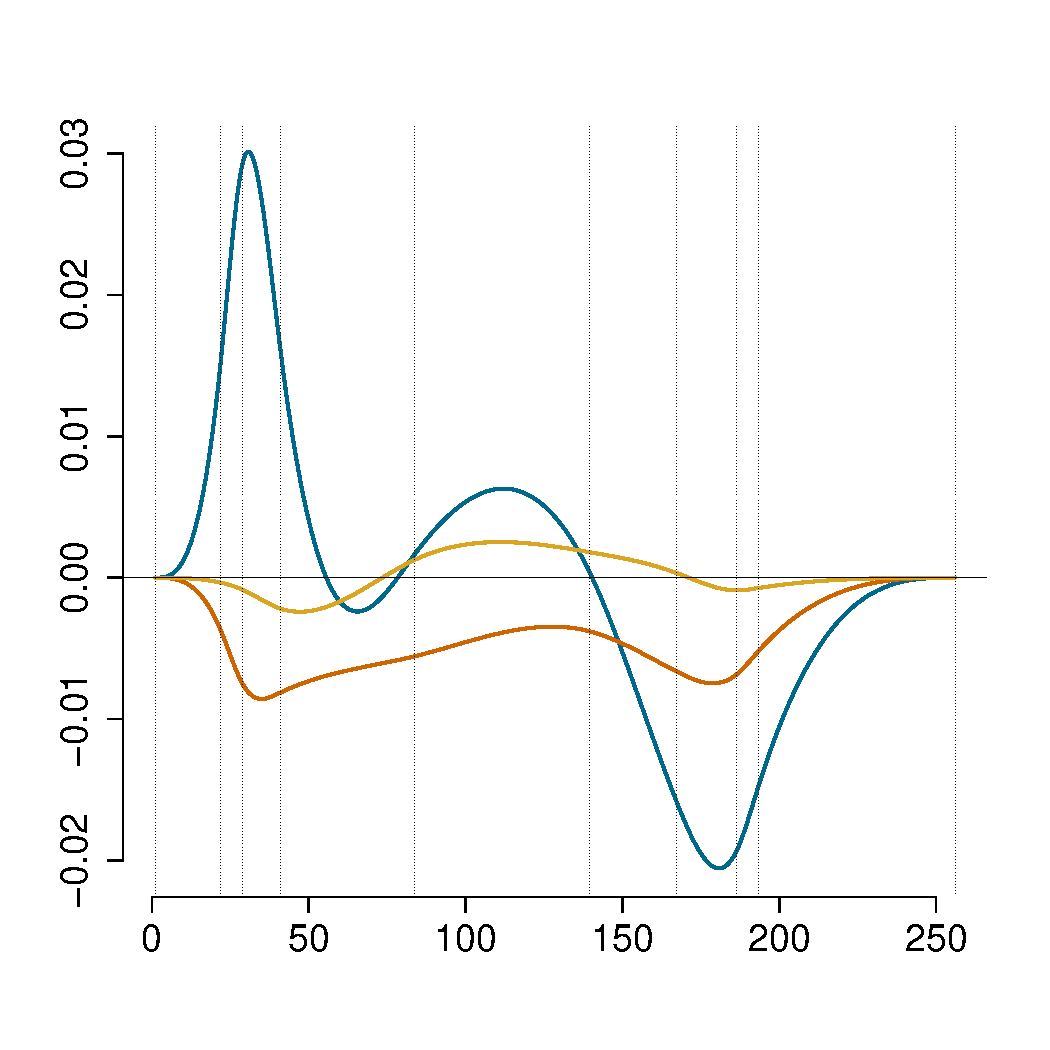
\includegraphics[width=0.5\linewidth]{figures/Fig5RightEigenFuncWine.pdf}
    \caption{ \emph{Left:} One sample of the data (blue curve), the data projected onto splinets (yellow curve) built over a set of selected knots, with the location of the knots indicated by vertical dashed lines, and the data decomposed using only the first eigenfunction (orange curve); \emph{Right:} the first three eigenfunctions scaled by the square roots of their corresponding eigenvalues.}
    \label{fig:eigen}
\end{figure}

The extracted principal components enable the identification of significant spectral differences between the samples, offering a more interpretable and efficient representation. The \code{plot()} function is then used to visualize both the original and projected data, as well as the principal components. The detailed plotting code can be found at { wine data example package vignette page } \url{https://ranibasna.github.io/R-Splinets/articles/FunctionalPrincipalValueDecomposition.html}.

This approach, leveraging the flexibility and efficiency of the \code{Splinets} package, provides a robust framework for analyzing functional wine spectra, ensuring that essential spectral features are preserved without overfitting.
Figure \ref{fig:eigen} (\emph{Left})  shows a sample from the dataset, comparing the original wine data (blue curve), the data projected onto splinets over the selected knots (yellow curve), and the data decomposed and reconstructed using only the first eigenfunction (orange curve). The vertical dashed lines indicate the locations of the selected knots. Figure \ref{fig:eigen} (\emph{Right})  shows the first three eigenfunctions scaled by the square roots of their respective eigenvalues.

\vspace{-.13cm}
\section{Classification problem - a case study using  \pkg{Splinets}}
\vspace{-.22cm}
The package  \pkg{Splinets} provides a comprehensive toolbox to analyze functional data. 
However, for a specific goal, one has to form a workflow that assures all steps have been performed to form the final conclusions following the analysis. 
Here, we introduce a workflow for the classification problems.
The focus here is on functional data that have a one-dimensional domain. 
In the future, we plan to extend the analytical tools to functional data with domains in higher dimensions such as images, movies, etc. 
For this reason, we have chosen a classic data set of images; however, our approach to their two-dimensional nature involves converting them into functions of one argument; for a more detailed discussion of the 2D extensions see \citep{Basna:2024aa}.
Before introducing the actual workflow, we explain the fundamentals of our methodology, highlighting the innovations that are specific to our use of spline spaces. 

\vspace{-.13cm}
\subsection{Methodology} \vspace{-.22cm}

In our approach to the classification of functional data, we first search for a suitable functional space of splines that captures important features of the data while maintaining a low dimensionality. These two seemingly opposing goals—fidelity and parsimony—must be balanced to ensure both efficiency and precision.

The main idea is to place knots in locations where the reduction in total squared error of the data approximation by 0-\code{degree} splines is largest. One implementation of this idea is available in the \pkg{ddk} package, written in R and accessible on GitHub: \url{https://github.com/ranibasna/ddk}, as discussed in \citep{basna2022data}.

For classification, spline spaces are selected separately for each class. The training data are then projected into the respective spaces, and these projections are referred to as functional data points. Functional principal component analysis (FPCA) is performed on the functional data points for each class in the training set. Specifically, the means are calculated for each class, and the centered data is decomposed into eigenvalues and eigenfunctions, yielding a spectral decomposition for each class separately.

This process involves estimating the eigenvalues ${\lambda_{i1}> \lambda_{i2} >\dots > \lambda_{in_i}}$ for the $i$th class, along with the corresponding set of eigenfunctions ${e_{i1}, e_{i2},\dots, e_{in_i}}$, where $n_i$ is the number of eigenfunctions for class $i$, and $i=1, 2, \dots, K$, with $K$ representing the number of classes. A validation method is used to determine the optimal number of eigenvalues and eigenfunctions. Theoretical validation of the spectral decomposition is through Karhune-Lo\`eve's representation of the functional data which states that a function in each class is sampled independently from the following model 
%%%%%%%%%%%%
\begin{align}
\label{eq:spectdec}
X_i(t)=\mu_i(t) +\sum_{k=1}^\infty \sqrt{\lambda_{ki}} Z_{ki} e_{ki}(t),\, i=1,\dots, K,  
\end{align}
%%%%%%%%%%%%
where $Z_{ki}$'s, mean-zero variance-one variables that are uncorrelated within a class and independent between classes. 

Subsequently, each original discretized data point, say $x_l$, from a test set is projected onto all $K$ spline spaces based on the original knot selection per class. 
Thus one obtains $K$ functional data points $f_{li}$, $i=1,\dots, K$. 
The core principle of classification is to determine how closely the $f_{li}$ test data point matches the projection to the eigenspaces for a given class. The mathematical techniques used in this process for image data include feature extraction, dimensionality reduction, and classification algorithms, which are used to obtain meaningful information from functional data points and classify them efficiently. 
Let us describe this classification procedure in some further detail.

The first step involves computing the mean for each of the ten classes using our training data sets. 
For a given class such a mean function of all elements in the training set belonging to the $i$th class is denoted by $\hat \mu_i$ and is viewed as an estimated value of $\mu_i$.
It is obtained by projection of the averaged data per class into a space of splines that has been determined by the knot selection process specifically for the mean.


For each original data point $x_l$ in the test set, one evaluates its representations $f_{li}$, $i=1,\dots, K$ in the spline spaces corresponding to each class.
Our objective is to assess the proximity to each of the $K$ classes by projecting $f_{li}-\hat \mu_i$ onto the eigenspaces (the space spanned by eigenfunctions) corresponding to that class. 
Thus, we obtain $K$ distinctive projections. We denote them by $\hat{f}_{l1},\hat{f}_{l2}, \dots, \hat{f}_{lK}$. Explicitly,
\begin{equation}
\label{eq:eigennu}
 \hat{f}_{li} =\hat \mu_i + \sum_{j=1}^{n_i} \langle f_{li}-\hat\mu_i,\hat e_{ji} \rangle \hat e_{ji},\, i=1,\dots, K   
\end{equation}
where $\langle\cdot \rangle$ stands for the inner product in the functional spaces, i.e. integral over the product of two functions, and $\hat e_{ij}$ are estimates of eigenfunctions $e_{ij}$ obtained in the training phase and discussed above. 
Formally, we obtain the following spectral decompositions
$$
f_{li}=\hat f_{li} +\hat\varepsilon_{li},
$$
where $\hat\varepsilon_{li}$ is the residual of the projection.
If the functional point $x_l$ belongs to the $i$th class and $\hat \mu_i$ and $\hat e_{ij}$ are approximately equal to the true values, we would have based on \eqref{eq:spectdec}:
\begin{align*}
\hat\varepsilon_{li}
\approx 
\sum_{j={n_i}+1}^\infty \sqrt{\lambda_{ki}} Z_{ki}  e_{ji}(t),
\end{align*}
which should be rather small in the squared norm $\|\cdot\|$ of the functional spaces. 
Indeed, we have
$$
\|\hat\varepsilon_{li}\|^2\approx
\left \|
\sum_{j={n_i}+1}^\infty \sqrt{\lambda_{ki}} Z_{ki} e_{ji}
\right \|^2
=
\sum_{j=n_i+1}^\infty \lambda_{ki} Z_{ki}^2 
$$
 and thus 
 $$
 \mathbb E (\|\hat\varepsilon_{li}\|^2)
 \approx
 \sum_{j={n_i}+1}^\infty \lambda_{ki}
 ,
 $$ 
 which can be made small as long as the selection of $n_i$ targets values so that
$ \sum_{j=1}^\infty \lambda_{ji} \approx   \sum_{j=1}^{n_i} \lambda_{ji}$. 

On the other hand, if $x_l$ does not belong to the $i$th class, the residual $\hat\varepsilon_{li}$ should be large, given that the classes are sufficiently distinguished by projections to the eigenspaces of their largest eigenvectors.   
This justifies the following classification rule 
\begin{equation}
    \label{eq:class}
    I(x_l)=\mathop{\rm arg\, min}_{i=1,\dots,K}\|\hat \varepsilon_{li}\|=\mathop{\rm arg\, min}_{i=1,\dots,K}\|x_l -\hat f_{li}\|,
\end{equation}
where $I(x_l)$ stands for the chosen class and $x_l$ is treated as a piecewise constant function. 
One can enhance the outcome of classification by providing the squared normalized distances
\begin{equation}\label{eq:weights}
\left(w_1^l,\dots, w_K^l\right)=\frac{\left(\|x_l -\hat f_{l1}\|^2,\dots, \|x_l-\hat f_{lK}\|^2\right)}{\sum_{i=1}^K \|x_l-\hat f_{li}\|^2}.
\end{equation}

\noindent\emph{Remark 1.}
This rule may be improved to account for the classes that differ not by eigenvectors but by the corresponding eigenvalues. 
Namely, one could consider the path of residuals over an increasing number of eigenvectors and consider the sizes of the residuals along this path. 
We do not investigate this enhancement of the proposed classification.

Having outlined the classification procedure, the pivotal role of selecting the appropriate eigenvalues/eigenfunctions for each class becomes evident. These hyper-parameters have a great impact on our classification results.
To enhance our classification's precision, we ascertain the ideal number of eigenvalues or eigenfunctions. Using the validation set technique, our primary objective is to identify the optimal count of eigenvalues/eigenfunctions. 

\vspace{-.13cm}
\subsection{Workflow}\vspace{-.22cm}
We describe, step-by-step, the workflow for the above-described methodology and, along with this, we perform these steps on the well-known Fashion MNIST dataset. The data set consists of a training set of 60,000 examples and a test set of 10,000 examples of Zalando's article images. The test dataset is divided into two distinct subsets: the validation dataset and the test dataset. Each data entry is represented by a grayscale image of $28 \times 28$ pixels. 
 The problem can be viewed as a classification problem on the $784$-dimensional Euclidean space.
Items belong to one of 10 types of clothing, such as shoes, dresses, etc. The name of each class and its corresponding label are: \emph{0 -- T-shirt/top, 1 -- Trouser, 2 -- Pullover, 3 -- Dress, 4 -- Coat, 5 -- Sandal, 6 -- Shirt, 7 -- Sneaker, 8 -- Bag, 9 -- Ankle boot}.

\begin{figure}[t!]
  \centering
\raisebox{-0mm}{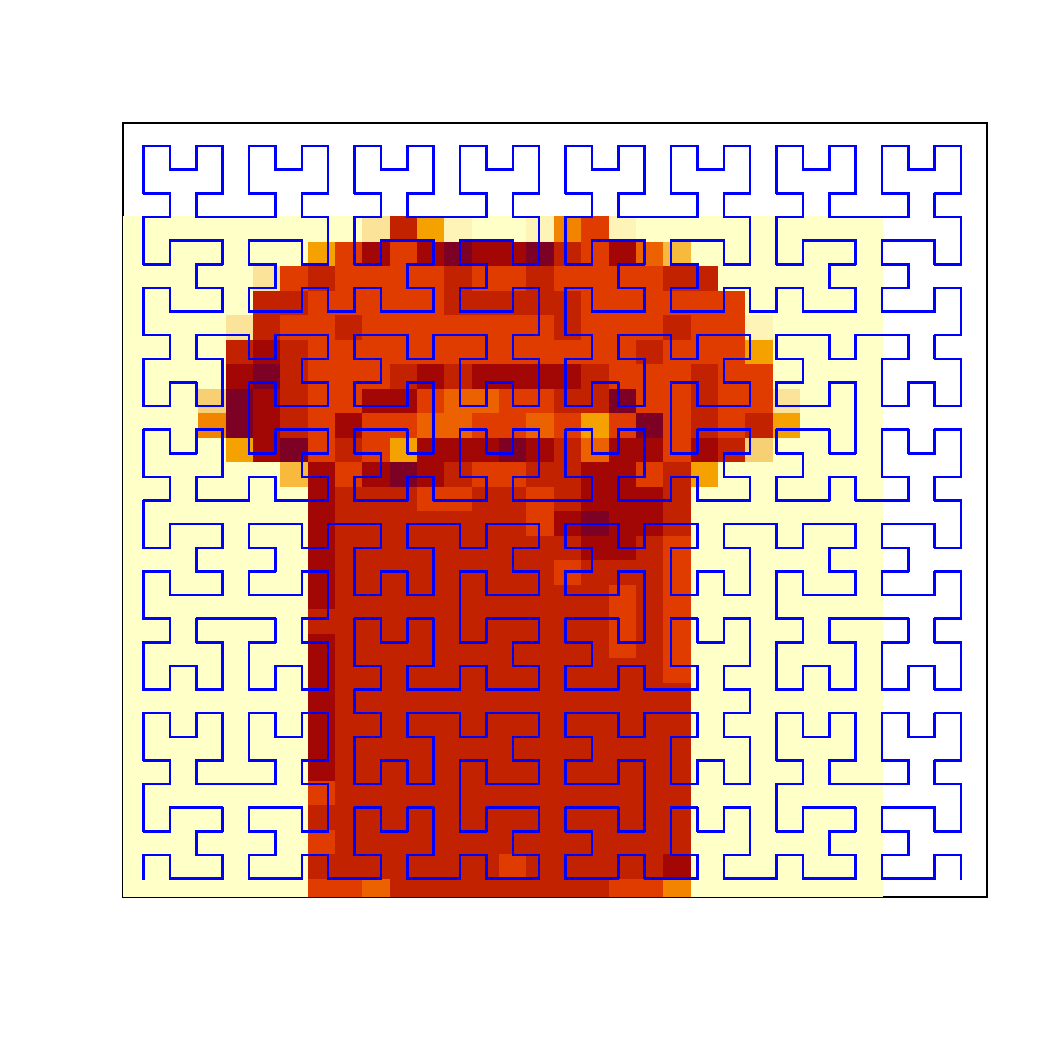
\includegraphics[width=0.32\textwidth]{figures/Fig6LeftT-shirt.pdf}} \hspace{-2mm}
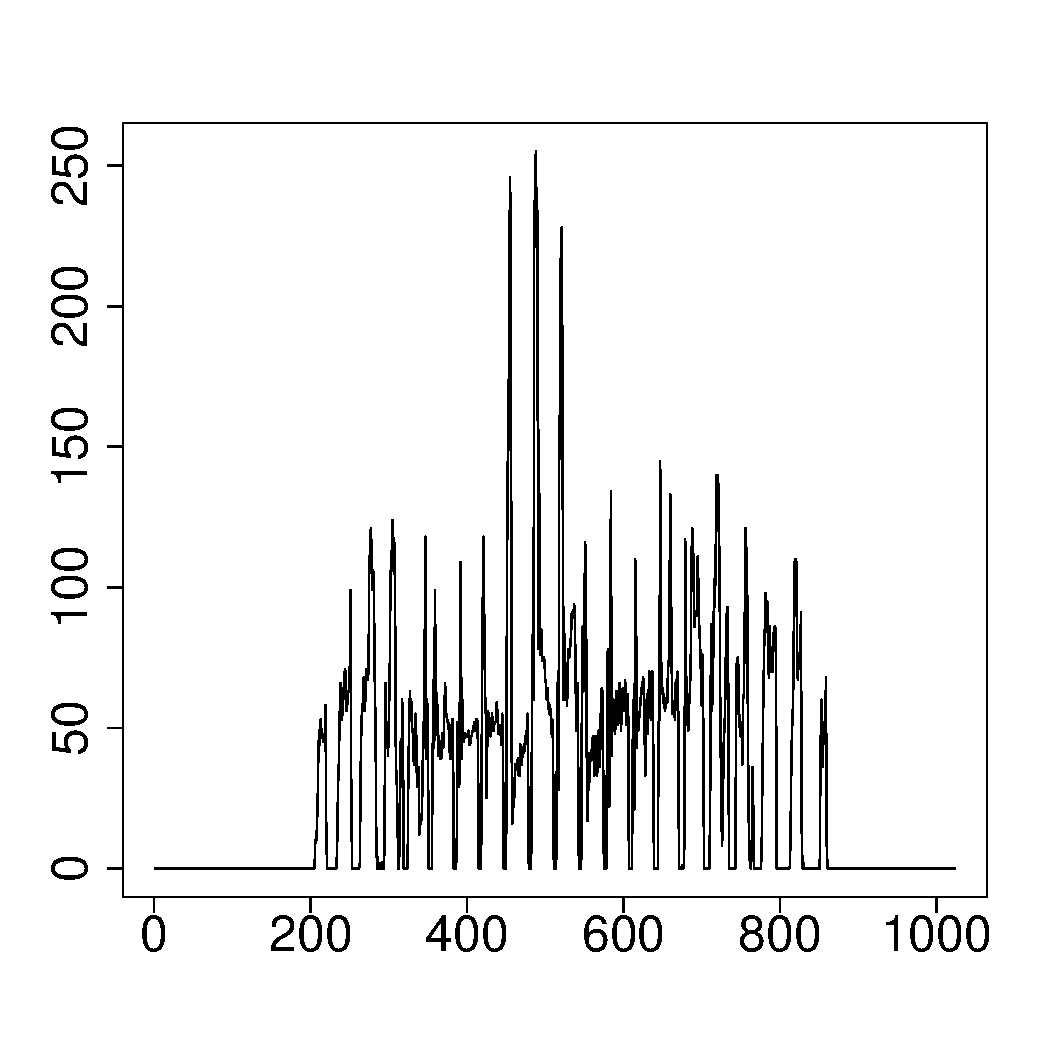
\includegraphics[width=0.33\textwidth]{figures/Fig6MiddleT-shirt.pdf}
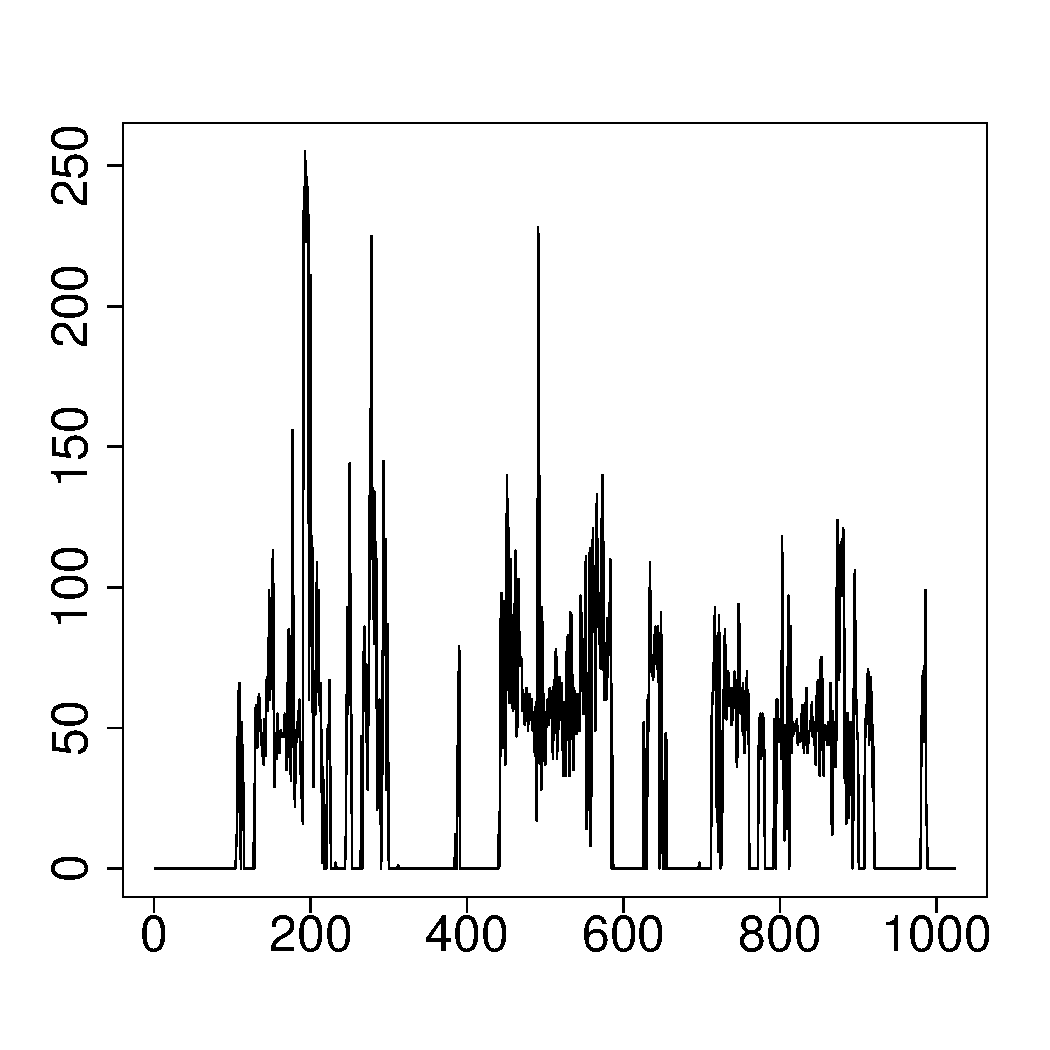
\includegraphics[width=0.33\textwidth]{figures/Fig6RightT-shirt.pdf}
  \caption{\footnotesize One- and two-dimensional representation of a  T-shirt . \emph{ Left:} original image with the Hilbert curve laid over;
  \emph{ Middle:} column-major order representation; 
  \emph{ Right:} Hilbert curve representation.}
  \label{HC}
  \end{figure}

\vspace{-.13cm}
\begin{enumerate}[leftmargin=0.2cm]
    \item{\bf Data preparation:} In this segment of the workflow, the package \pkg{Splinets} is not used but the way we represent and preprocess our data plays a critical role in subsequent analyses and outcomes. 
    The remaining steps of the workflow assume that the data represent discretized functions, i.e. are matrices of columns representing arguments and values of the functional data. 
    Two variants of this format are allowed: one with the common arguments for all data points, where the vector of arguments stands as the last column; the second one allows different arguments for different data points, in which the input should be a list of two-column matrices, with the vector of the arguments as the first column and the vector of the corresponding values as the second one. 
    We note that in the second case, it is allowed to have a varying number of rows in the elements of the list. 

    Once the data are properly formatted, it should be divided into three parts. The first and largest part (typically at least $50\%$ of the data) constitutes the training data, and the remaining are split into two, the validation and testing. 
    Alternatively, one can perform training and cross-validation on a data set of size, for example, $75\%$, and test the approach on the remaining testing portion of the data.
    
    \noindent\textbf{Example:} (Fashion MNIST dataset).
     For the Fashion MNIST dataset, we deal with two-dimensional images, and transforming the data to one dimension is a critical process in which information will be lost. One of the tasks, we settled with the analysis of this data set is to compare different approaches to this transformation process. For this reason, we elucidate our approaches to data representation and transformation.
 
    Images are typically represented as matrices of pixels, where the value of each matrix element indicates the color and intensity of the respective part of the image.
    The matrices need to be transformed into vector form. A prevailing approach for such a transformation involves stacking the image's columns (or rows) consecutively to create a vectorized representation. However, this technique often neglects the local spatial correlations existing between image pixels, ensuring only the preservation of vertical (or horizontal) correlations.

    To more effectively retain these local correlations, we turn to the Hilbert curve transformation. 
    A Hilbert curve is a continuous fractal space-filling curve that traverses every point in a square grid sized to any 2-power magnitude.  For a detailed discussion of Hilbert curves, we refer to \citep{bader2012space}. Hilbert curves are particularly interesting for their ability to group pixels locally, see also R-package  \pkg{gghilbertstrings} on CRAN \citep{gghilbertstrings}. 
    The additional materials accompanying the paper show the explicit definition of the Hilbert curve used for our data obtained from the R-code of the Hilbert space-filling algorithm.
    This specific case of the Hilbert curve is shown in Figure~\ref{HC} \emph{ (Left)} laid over the picture of a shirt. 

    Given that our image dimensions do not align with a 2-power magnitude, we have implemented zero padding, adjusting the image to a $2^5\times 2^5$ pixel matrices. Figure~\ref{HC} presents two illustrative examples from the MNIST dataset: a shirt and a boot. The middle illustrations provide vectorized representations of these items, derived from consecutively stacking image columns. The right-hand-side depictions visualize vectors formed through the Hilbert space-filling curve. It is easy to notice that the locality-preserving properties of Hilbert's curve make the vectorization based on it a better choice in comparison to the column-wise vectorization.
    We also see that the Hilbert curve vectorization lead to more sparse data which could be accounted for using disjoint-interval domains featured by the package, which would lead to more efficient computations.
    However, this aspect of the data has not been implemented as we did not face any major computational burden in our studies. 
    \item {\bf Projection into spline spaces built on selected knots:} In this step, we consider $K$ distinct third-{  degree} data-driven splinet bases, {each built on knots specifically chosen for the corresponding class among the $K$ available. The number of knots for each class, as well as their placement, is determined using the DDK algorithm to effectively capture changes in the data.} We then project the discrete training data points onto these splinets, constructed based on the class-specific knots.
    We considered separated spaces for the mean discrete data and the centered discrete data. 
    We note that since the knots for the mean data are a subset of the knots for the centered data, the projections of the means are in the space of the projections of the centered data. However, they are not the same as their projections of the centered data space. 


\begin{figure}[t!]
\begin{center}
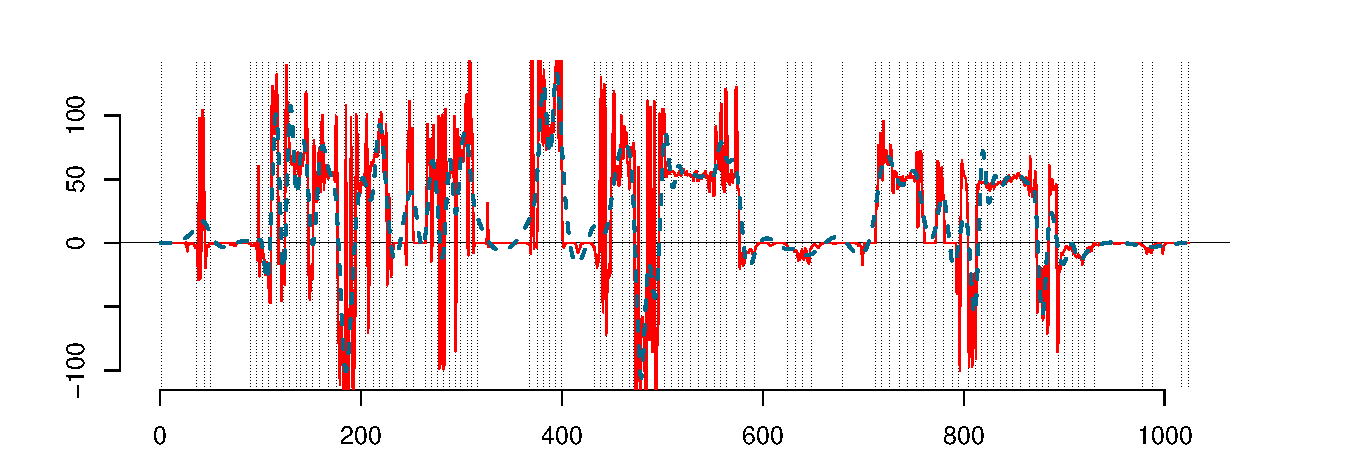
\includegraphics[width=0.9\textwidth]{figures/Fig7T-shirtfit.pdf}  
\end{center}
\caption{\footnotesize  Fitting the centered `T-shirt' by a spline with selected knots  marked by vertical dotted lines.}
  \label{fig:KnotSelMean}
\end{figure}
These projections establish an isomorphism between the Euclidean vectors made of coefficients of the projection and the space of splines into which the original data have been projected. 
More specifically, if $N_i$ is the number of knots chosen of the $i$th class and $k$ is the {  degree} of the splines, then the splines spanned on these knots constitute a $N_i-k-1$-dimensional Hilbert space with $N_i-k-1$ elements of the corresponding splinet so that 
\begin{equation}
\label{eq:isom}
x_l\stackrel{\tiny proj}{\longmapsto} f_{li} \stackrel{\tiny isom}{\longleftrightarrow} \mathbf a_{li}\in \mathbb R^{N_i-k-1},
\end{equation}
where $x_l$ is either the original centered discrete data point, $f_{li}$ is the corresponding functional data point when projected on the knots selected for the $i$th class, $\mathbf a_{li}$ is the vector of coefficients corresponding to the splinet expansion of $f_{li}$. 
This isomorphism allows us to perform the next part of the analysis simply by doing standard multivariate analysis on $\mathbf a_{li}$'s.
The projection process is facilitated using the {\tt project()} functions in the R-\pkg{Splinets} package.
Other functions of the package assist exploration and visualization of various features of $f_{li}$'s.
%%%%%%%%%%%%%%%%%

\noindent\textbf{Example:} (Fashion MNIST dataset, cont.). The original images that were transformed through the Hilbert curve transform to the 1D discrete data are next projected to spline spaces, { where the number of knots for the respective classes are 
    $$
    (N_1,N_2,N_3,N_4,N_5,N_6,N_7,N_8,N_9,N_{10})=(106 , 78, 100 ,86, 94, 100, 106,  78, 128, 102).
    $$ }
    Considering the number of knots and since we consider the third {  degree}  splines the dimension of the spline spaces are to be computed and put here according to the formula $(N_i-4)$. We note the initial dimension reduction from $784$ to the reported values of the given knot numbers in the classes. Additional further dimension reduction will be achieved through FPCA later on in the workflow.  We see the projection of the `T-Shirt' mean and an example of a  centered `T-Shirt' in Figure~\ref{fig:KnotSelMean}~\emph{(Top-Middle)}. The locations of knots for these two cases are shown by vertical dashed lines.     
    
\begin{figure}[t!]
  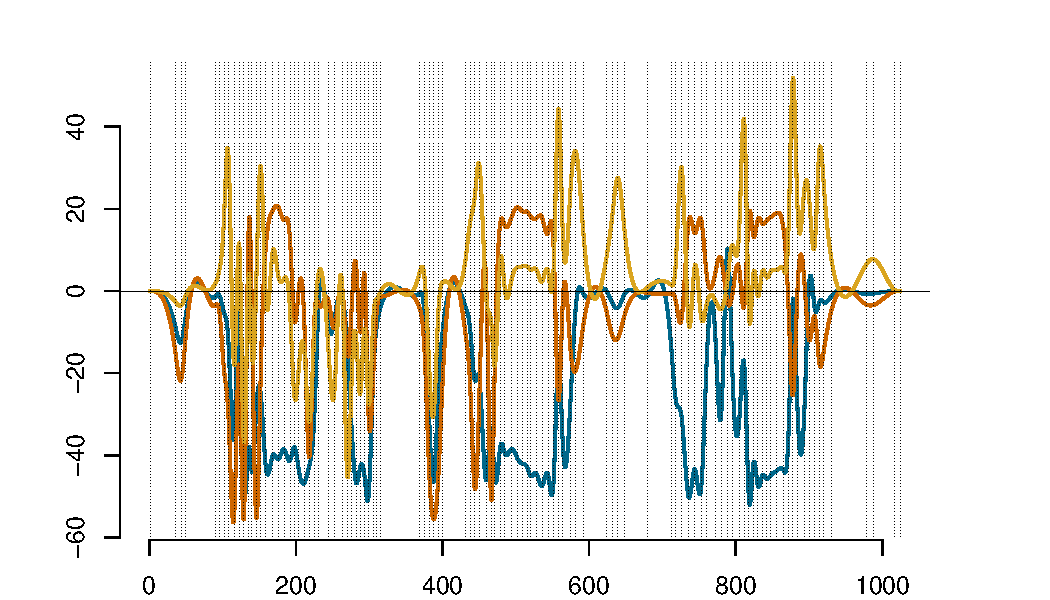
\includegraphics[width=0.55\textwidth]{figures/Fig8TopLeft.pdf}\hspace{-10mm}
    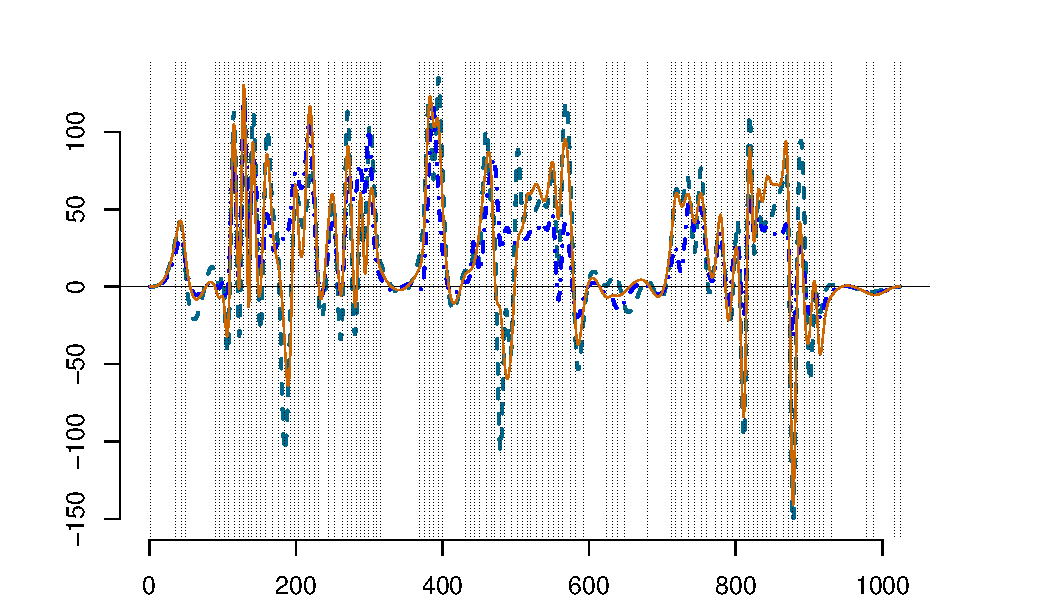
\includegraphics[width=0.55\textwidth]{figures/Fig8TopRight.pdf}\hspace{-5mm}\\
  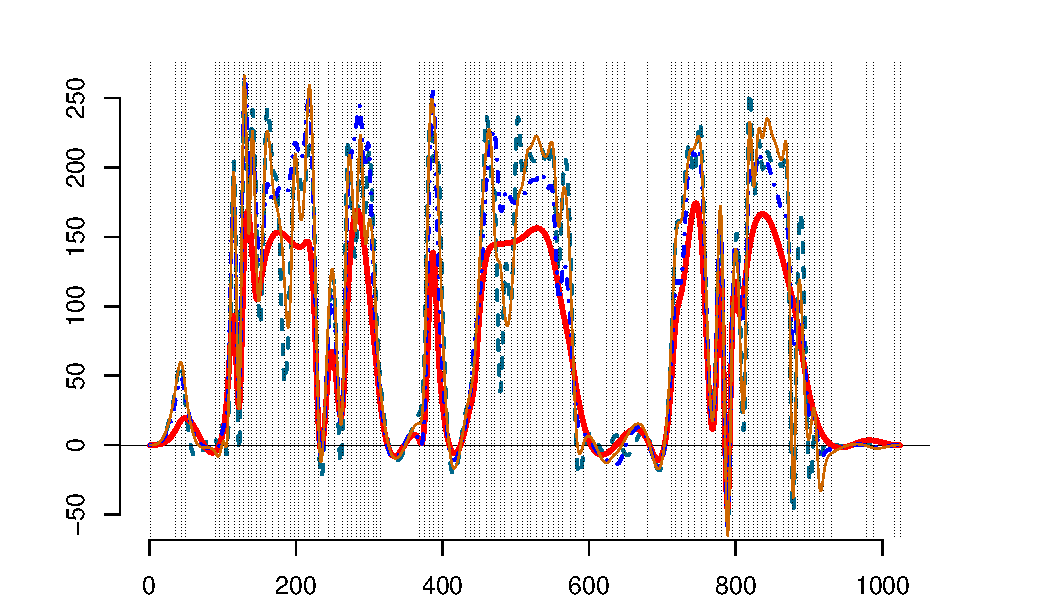
\includegraphics[width=0.55\textwidth]{figures/Fig8BottomLeft.pdf}\hspace{-10mm}
  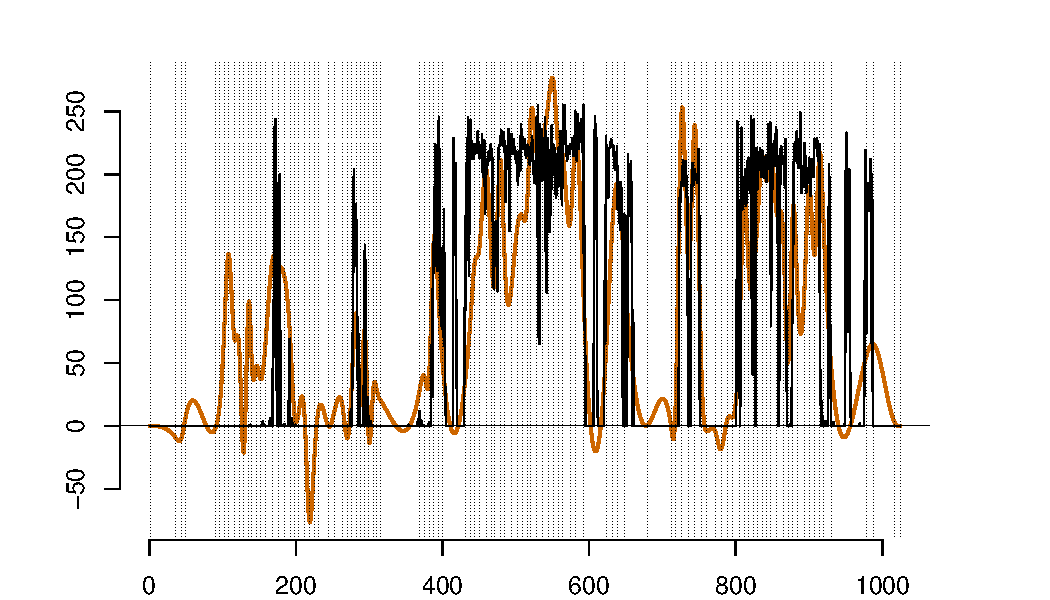
\includegraphics[width=0.55\textwidth]{figures/Fig8BottomRight.pdf}\hspace{-5mm}
  \caption{\footnotesize The spectral decomposition of the training data. 
  \emph {Top-Left:} The first three eigenfunctions for the `T-shirt' class scaled by the square roots of the respective eigenvalues, 
  \emph{ Top-Right:} Two approximations of the centered functional `T-shirt' data point \emph{ (NavyBlue-Dashed Line)}: 1) by the first three eigenfunctions \emph{ (Blue-DottedDashed Line)} ; 2) by the first twenty eigenfunctions \emph{ (Orange-ThinSolid Line)},
  \emph{ Bottom-Left:}
  The same approximation but centered around the `T-Shirt' class mean $\hat \mu_1$ \emph{ (Red-ThickSolid Line)},
  \emph{ Bottom-Right:}
  Projection of a 'Boot' data point to the 'T-Shirt' spectrum with 20 eigenfunctions after centering around the 'T-Shirt' class mean, the  `Boot' data point \emph{ (Black-Rough Line)} vs. its projection \emph{ (Orange-Solid Line).}
}
  \label{KS_EigenFunctions}
  \end{figure}

\item {\bf FPCA on training data:}
 To facilitate the classification procedure in the next step but also to gain a deeper understanding of the complexity of the data, the FPCA is performed within each class of the functional data points of the training set. In this task, one utilizes the isometry given in \eqref{eq:isom}, and first the sample covariance matrix $\boldsymbol \Sigma_i$ is evaluated
 $$
 \boldsymbol \Sigma_i = \overline{\mathbf a_{.i}\mathbf a_{.i}^\top} -\overline{\mathbf a_{.i}}\,\,\overline{\mathbf a_{.i}}^\top,
 $$
 where averaging $\overline{\cdot}$ is made within the class $i$ of the training data. 
One simply applies \code{cov()} on the matrix of column vectors $\mathbf a_{li}$'s. 
 Then the spectral decomposition of $\boldsymbol \Sigma_i$ into eigenvalues and eigenvectors is performed using \code{eigen()} of the R -\emph{ base} package. 
 The obtained eigenvectors correspond to eigenfunctions through the isometry.
 
\noindent\textbf{Example:} (Fashion MNIST dataset, cont.).
  This rather standard step when performed on cloth image classes is illustrated in Figure~\ref{KS_EigenFunctions}. The first three eigenfunctions of `T-shirts' scaled by the square roots of the respective eigenvalues are shown in the \emph{ (top-left)} graph and projections to the spaces based on 3 and 20 eigenfunctions are presented in the remaining graphs including the projection of  `Boots' to the `T-Shirt' space, the \emph{ (bottom-right)} graph.

  \item {\bf Determining the significant eigenfunctions:}
In this step, the classification procedure \eqref{eq:class} as a function of the number of considered eigenfunctions is implemented.
Then the number $n_i$ of the eigenfunctions for the $i$th class is based on its accuracy on the validation data set.
In Figure~\ref{KS_EigenFunctions}~\emph{ (Bottom)}, we see the illustration of the classification principle. 
There are shown approximation of two data points, a `T-Shirt' \emph{ (Left)}, and a `Boot' \emph{ (Right)}, based on the projection to 20 eigenvalues in the 'T-Shirt spline space. It can be seen clearly that the approximation of 'T-shirt' is better than the approximation of `Boot'. 
The functional $L_2$-norm of the functional spaces can be utilized to measure the approximation. 

The approach to data classification relies on projecting the data into a subspace defined by a set of numbers $n_i$, $i=1,\dots, K$, of eigenfunctions of the distinct classes.
We can see from \eqref{eq:eigennu} and the classification rule \eqref{eq:class} that if $n_i$'s are taken too big, then it may result in overfitting of the data and a smaller dimension reduction, on the other hand, if the values are too small the precision of distinguishing the features in the data of different classes may be not sufficient. 
In this framework, the numbers of eigenfunctions for individual classes are of paramount significance and are treated as hyper-parameters.
The $n_i$'s, $i=1,\dots,K$ are chosen through the following cross-validation procedure. 

From the training data, from each class, we exclude at random $10\%$-data points, denoted by $\mathcal C_i$, $i=1,\dots,K$. 
Consider the remaining $90\%$ for the $i$th class and build spectral decomposition of the data as explained in the previous step.
Set the initial vector of numbers of the eigenvalues $\mathbf n^0=(n^0_1,\dots,n_{10}^0)$ in each class. For example, we can set it to zero to start with the classification based only on the mean $\hat \mu_i$, i.e. the closest mean decides for the class to which a data point belongs to. 
Let the classification distances (evaluated through \eqref{eq:weights}) for a given discrete data point $x$ be denoted by 
$$
\mathbf w(x,{\mathbf n^0})=\mathbf w(x;n^0_1,\dots,n_{10}^0).
$$
Evaluate classification success rate through
$$
\mathbf s({\mathbf n^0})=\left(\frac{\sum_{x\in \mathcal C_1} w_1(x,\mathbf n^0)}{|\mathcal C_1|},\dots,\frac{\sum_{x\in \mathcal C_K} w_K(x,\mathbf n^0)}{|\mathcal C_K|} \right).
$$
where $|\mathcal C_i|$ is the number of elements in $\mathcal C_i$, or through the classification accuracy rate
$$
\mathbf a({\mathbf n^0})=\left(\frac{\#\{x\in \mathcal C_1; I(x,\mathbf n^0)=1\}}{|\mathcal C_1|} ,\dots,\frac{\#\{x\in \mathcal C_K; I(x,\mathbf n^0)=K\}}{|\mathcal C_K|} \right).
$$
Small values in $\mathbf s$ or large values in $\mathbf a$ indicate good classification. 
Thus, taking averages of these two vectors can be used to assess the overall quality of a classification rule. 
Since the accuracy $\mathbf a$ is more interpretable, we focus on it and denote the average of its entries by $\bar {\mathbf a}$. 

In general, the function $\mathbf n\mapsto \bar {\mathbf a}(\mathbf n)$ is a non-convex function of $K$ arguments, and our goal is to find its optimum when evaluated over the validation data set.  
We adopt a simple iterative marginal gradient method, where we increase by one that coordinates in $\mathbf n$ that produces the large increase in $\bar {\mathbf a}$. 
Allow for a specific number of negative increases $L$ and conclude with the location $\mathbf n_{opt}$ of the maximum over-searched path.  
The number $L$ is a hyperparameter and is data-specific. 
The algorithm is repeated by a number of random initial knot distributions and the final result is the maximum over these runs.
%%%%%%%%%
 \begin{figure}[t!]
  \centering
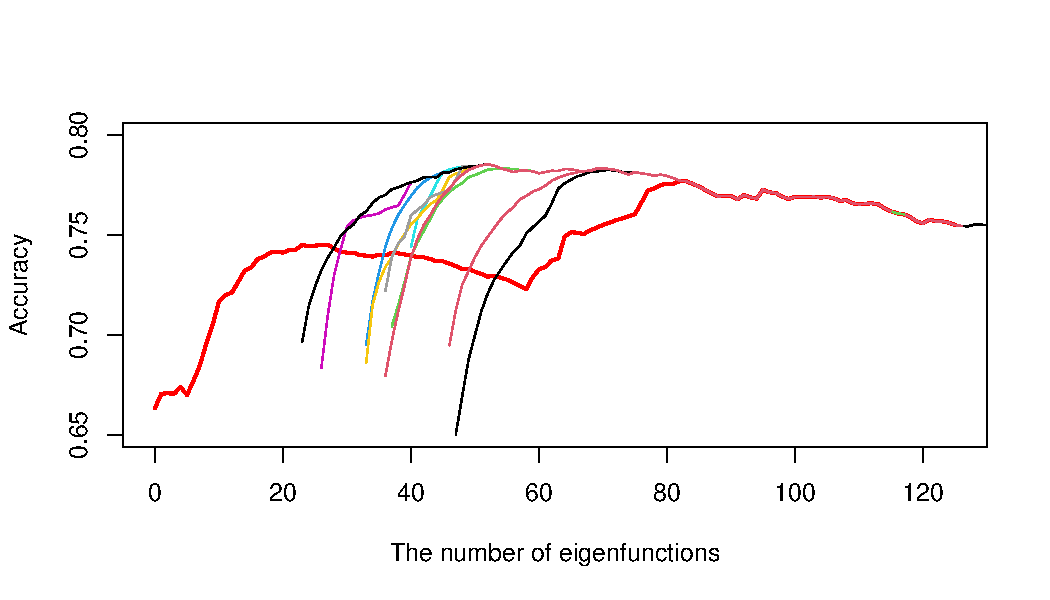
\includegraphics[width=0.75\textwidth]{figures/Fig9Left.pdf}\vspace{-1.5cm}\\
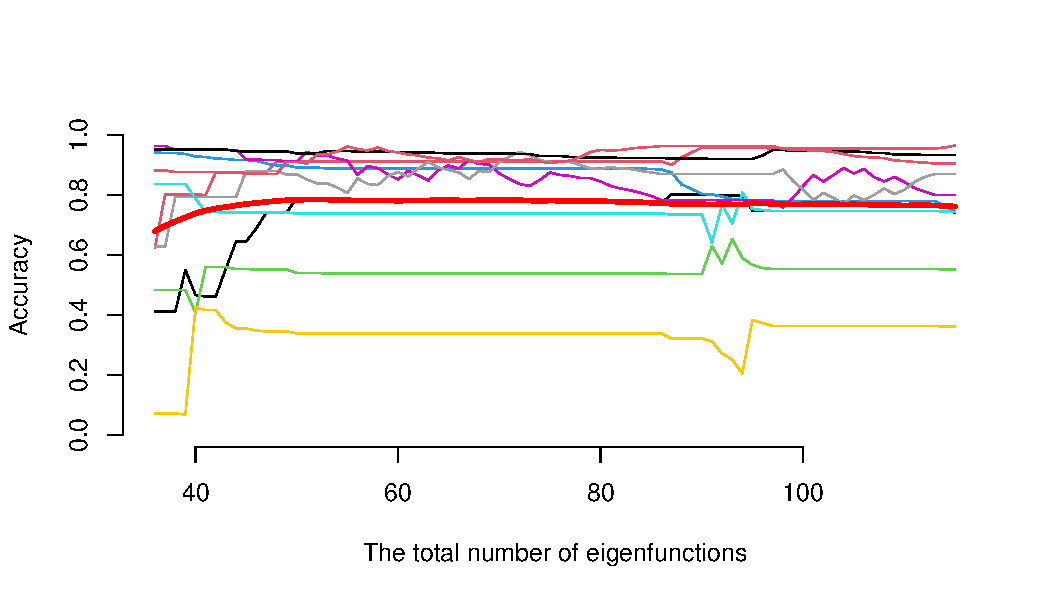
\includegraphics[width=0.75\textwidth]{figures/Fig9Right.pdf}\vspace{-0.4cm}

  \caption{\footnotesize Optimization of the accuracy function in the validation phase (Step 4). \emph{ Top:} The trajectory of the average accuracy along the initial optimization path (thick-line) together with subsequently chosen random samples of the initial $\mathbf n_0$ that are shown in thin-lines; \emph{ Bottom:} The class-wise accuracies (thin-lines) against the average accuracy (thick-line). `Pullovers' (green line) and `Shirts' (yellow line) are notoriously difficult to classify.  }
  \label{VAL}
  \end{figure}

\noindent\textbf{Example:} (Fashion MNIST dataset, cont.).
 In Figure~\ref{VAL} \emph{ (Top)}, the different trajectories of the accuracy obtained for randomly picked $\mathbf n_0$ are shown in thin-lines. The procedure was run on the validation set of the functional using the classification procedure \eqref{eq:class} (also used in the next step of the workflow). 
The baseline for the performance is made of the rates of correct classification per class when it is only based on the distance of a data point from the spline projection of the mean, i.e. $\|x-\hat \mu_i\|$, so no eigenfunctions are considered. 
The obtained rates of correct classification rates per class are 
$$
(0.67, 0.88, 0.33, 0.73, 0.66, 0.75, 0.23, 0.80, 0.76, 0.86)
$$
with the overall average performance of $66\%$ of correct classification.
From this, one sees that `Pullover' and `Shirt' seem to be difficult to classify. 
Overall accuracy is assessed using the approach as described above with random starting vector $\mathbf n_0$ of the initial allocation of the numbers of the eigenvalues in the class and searching for the optimal allocation.
The procedure is illustrated in Figure~\ref{VAL} \emph{ (Top)}, where several subsequent trajectories of the total accuracy are presented by the thin-lines against the initial selection, the thick-line.
In Figure~\ref{VAL} \emph{ (Bottom)}, the trajectories of the classwise accuracies and the average accuracies based on the above optimization procedure are presented. They lead to
the following numbers of significant eigenvectors $(  8,  4,  5,  6,  4, 8,  2, 4,  5, 6)$ for the ten cloth classes and, with this choice, the average accuracy in the validation process is $78.5\%$. We conclude that the original dimension of $784$ vectors has been reduced more than tenfold (based on the total number $52$ of all eigenfunctions). 
However, we also see that `Pullovers' (y and `Shirt' remain hard to classify, with the latter being properly classified less than $40\%$ of the time. 
The final classification based on the obtained sizes of the functional spaces is performed on the testing data set in the next step. 

\item {\bf Testing the classification procedure:}
This step is essentially repeating on the testing data set, most of the workflow except the validation steps used for the knot selection and deciding for the number of eigenfunctions. 
Thus for each data point $x_l$ in the testing sets, one projects it to ten functional spaces obtaining splines $f_{li}$, $i=1,\dots, K$. Those in turn are used to evaluate the classification rule \eqref{eq:class} and decide on the class of the object. 
In fact, in the algorithm, the following convenient representation of the squared distance between a discrete data point $x_l$ and its approximation $\hat f_{li}$ given in \eqref{eq:eigennu} is used 
$$
\|x_l-\hat f_{li}\|^2=\|x_l\|^2-\|f_{li}\|^2 + \|f_{li}-\hat \mu_i\|^2
-\sum_{j=1}^{n_i}\left| \langle f_{li}-\hat \mu_i,\hat e_{ji}\rangle\right|^2.
$$
The results are compared with actual class memberships and summarized in the confusion matrix and other standard measurements of efficiency. 

\noindent\textbf{Example:} (Fashion MNIST dataset, cont.).
The leading example illustrating the workflow is using Hilbert curve approach to transform from two-dimensional images to one-dimensional discrete data points.  
The classification method \eqref{eq:class} with optimally chosen numbers of eigenvectors was performed through all testing data points and several characteristics have been evaluated.
The average accuracy (over all classes) is $77.0\%$, which is close to the one in the cross-validation step and the classwise accuracies are 
$$
(73.4\%, 89.1\% ,52.3\%, 87.7\%, 72.0\% , 91.7\%, 32.9\%, 82.2\%, 94.5\%, 92.9\%),
$$
which are also consistent with the results in the cross-validation experiment seen in Figure~\ref{VAL}~\emph{ (Bottom)}. 

Another important summary is to report the averaged normalized distances $\bar{\mathbf w}$, of the elements of the class to their projection to that class and they are
$$
 (0.049, 0.049, 0.053, 0.046, 0.047, 0.051, 0.060, 0.033, 0.042, 0.030).
$$
We observe expected negative correlations with the accuracies. The values are significantly lower from $0.1$ (the case that the distance does not differentiate between classes) and are a major improvement over the original relative distances to the spaces. 

\item {\bf Final evaluation and conclusions:}
This part depends on the goal for which the classification procedure has been used and thus is case-specific. 
One may need simply a classification method and its accuracy, then little is needed beyond the details shared in the previous step.
%in which case not much is needed beyond what has been reported in the previous step. 
    It is also recommended to examine the statistics of misclassified data points and the features of these points as expressed by FPCA. 
    This may give insight into the reasons for failing to identify data points properly and, in consequence, give an idea of how the classification can be further improved. 
    If classification needs to be applied to some data without labels, then the classification should be run on it and summarized. 
    This workflow can also serve as a benchmark to compare various classification methods.
   %One can also use the above workflow to compare different classification methods.
   Then a comparison and a discussion should be carried out through reporting confusion matrices, along with other pertinent evaluation metrics. Again checking which data points have been misclassified can be important to see if a hybrid classification method could further improve the success rate.

\noindent\textbf{Example:} (Fashion MNIST dataset, cont.).
In our illustrative example, the goal was to show the workflow and the corresponding methodology. 
Since we focused on a single method, it is natural to present here more detailed characteristics of the method and comment on the obtained outcomes.
It is clear that the method performs poorly in classifying `Shirts' and, somewhat better, `Pullovers'.  We observe that a `Shirt' is often classified as a `T-Shirt' and a `Coat'. Additionally, a `Pullover' is often classified as a `Coat'. 
Generally, it seems that the main responsibilities for the misclassifications are the classes: `T-shirt', `Pullover', `Coat', and `Shirt'. 

To improve on the method one could try to use a lower {  degree} of splines that could help due to the noisiness of the Hilbert curve data points. 
By just looking at the data, it appears that the first-{  degree} splines should suffice.
Improving the search for an optimal number of eigenfunctions could be another possible source of improvement. 
We have seen that the performance from the validation step carries over to the testing results.
Thus, enhancing the validation process should lead to more accurate classification results.
Nevertheless, it seems that the achieved performance will be hard to significantly improve unless the full 2D character of the data is considered. 
This is planned in a future 2D extension of the spline-based method for the FDA. 




\begin{table}[h]
\centering
\caption{Confusion matrix}
\small
 \begin{tabular}{l r r r r r r r r r r}
 \toprule 
 \multicolumn{11}{c}{\bf TARGET}\\
 \bf PREDICT. &T-shirt & Trouser & Pullover & Dress & Coat & Sandal & Shirt & Sneaker &Bag &Boot\\
 \midrule
T-shirt& 73.4\% &0.8\% &4.5\% &4.6\% &0.8\% &0.0\% & 25.5\% &0.0\% &2.2\% & 0.1\%\\
Trouser& 0.1 & 89.1\% &0.3\% &1.7\% &0.1\% &0.0\% &0.0\% &0.0\% &0.0\% & 0.0\%\\
Pullover& 1.8\% &0.5\% & 52.3\% &1.5\% & 10.4\% &0.0\% &8.6\% &0.0\% &0.7\% & 0.0\%\\
Dress & 12.1\% &8.7\% &2.0\% & 87.7\% &8.4\% &0.0\% &8.9\% &0.0\% &1.2\% & 0.0\% \\
Coat & 0.3\% &0.6\% & 20.2\% &1.7\% & 72.0\% &0.0\% & 17.9\% &0.0\% &0.2\% & 0.0\%\\
Sandal & 0.7\% &0.0\% &0.0\% &0.1\% &0.0\% & 91.7\% &0.0\% &9.2\% &1.0\% & 3.3\%\\
Shirt & 5.0\% &0.1\% & 17.5\% &1.8\% &6.8\% &0.0\% & 32.9\% &0.0\% &0.0\% & 0.0\%\\
Sneaker & 0.0\% &0.0\% &0.0\% &0.0\% &0.0\% &4.7\% &0.0\% & 82.2\% &0.1\% & 3.7\% \\
Bag & 6.6\% &0.2\% &3.0\% &0.8\% &1.4\% &0.4\% &6.2\% &0.0\% & 94.5\% & 0.0\% \\
Boot & 0.0\% &0.0\% &0.2\% &0.1\% &0.1\% &3.2\% &0.0\% &8.6\% &0.1\% &92.9\%\\
\bottomrule
\end{tabular}
\label{tab:confusion}
\end{table}
\end{enumerate}

\vspace{-.13cm}
\subsection{Comparing different 1D-methods functional methods}\vspace{-.22cm}
We employ the proposed workflow to investigate how different methods of data preparation influence the efficiency of our classification method.
Our main goal is to assess the impact on the efficiency of two factors: the Hilbert curve-based transformation method and the data targeted knots selection.

 (that can be obtained, for example, by using DDK described in  \cite{basna2022data}). 
We put forward three distinct scenarios to be examined using our established workflow:
\begin{itemize}
    \item [S1:] Hilbert curve transformation with $100$ data-driven knot selections.
    \item [S2:] By-row data with $100$ data-driven knot selections.
    \item [S3:] By-row data with $100$ equidistant knots.
\end{itemize}
This choice ensures both the validity and fairness of our comparisons, thus enhancing the reliability and interpretability of our results. 

\begin{figure}[t!]
  \centering
\hspace*{-.8cm}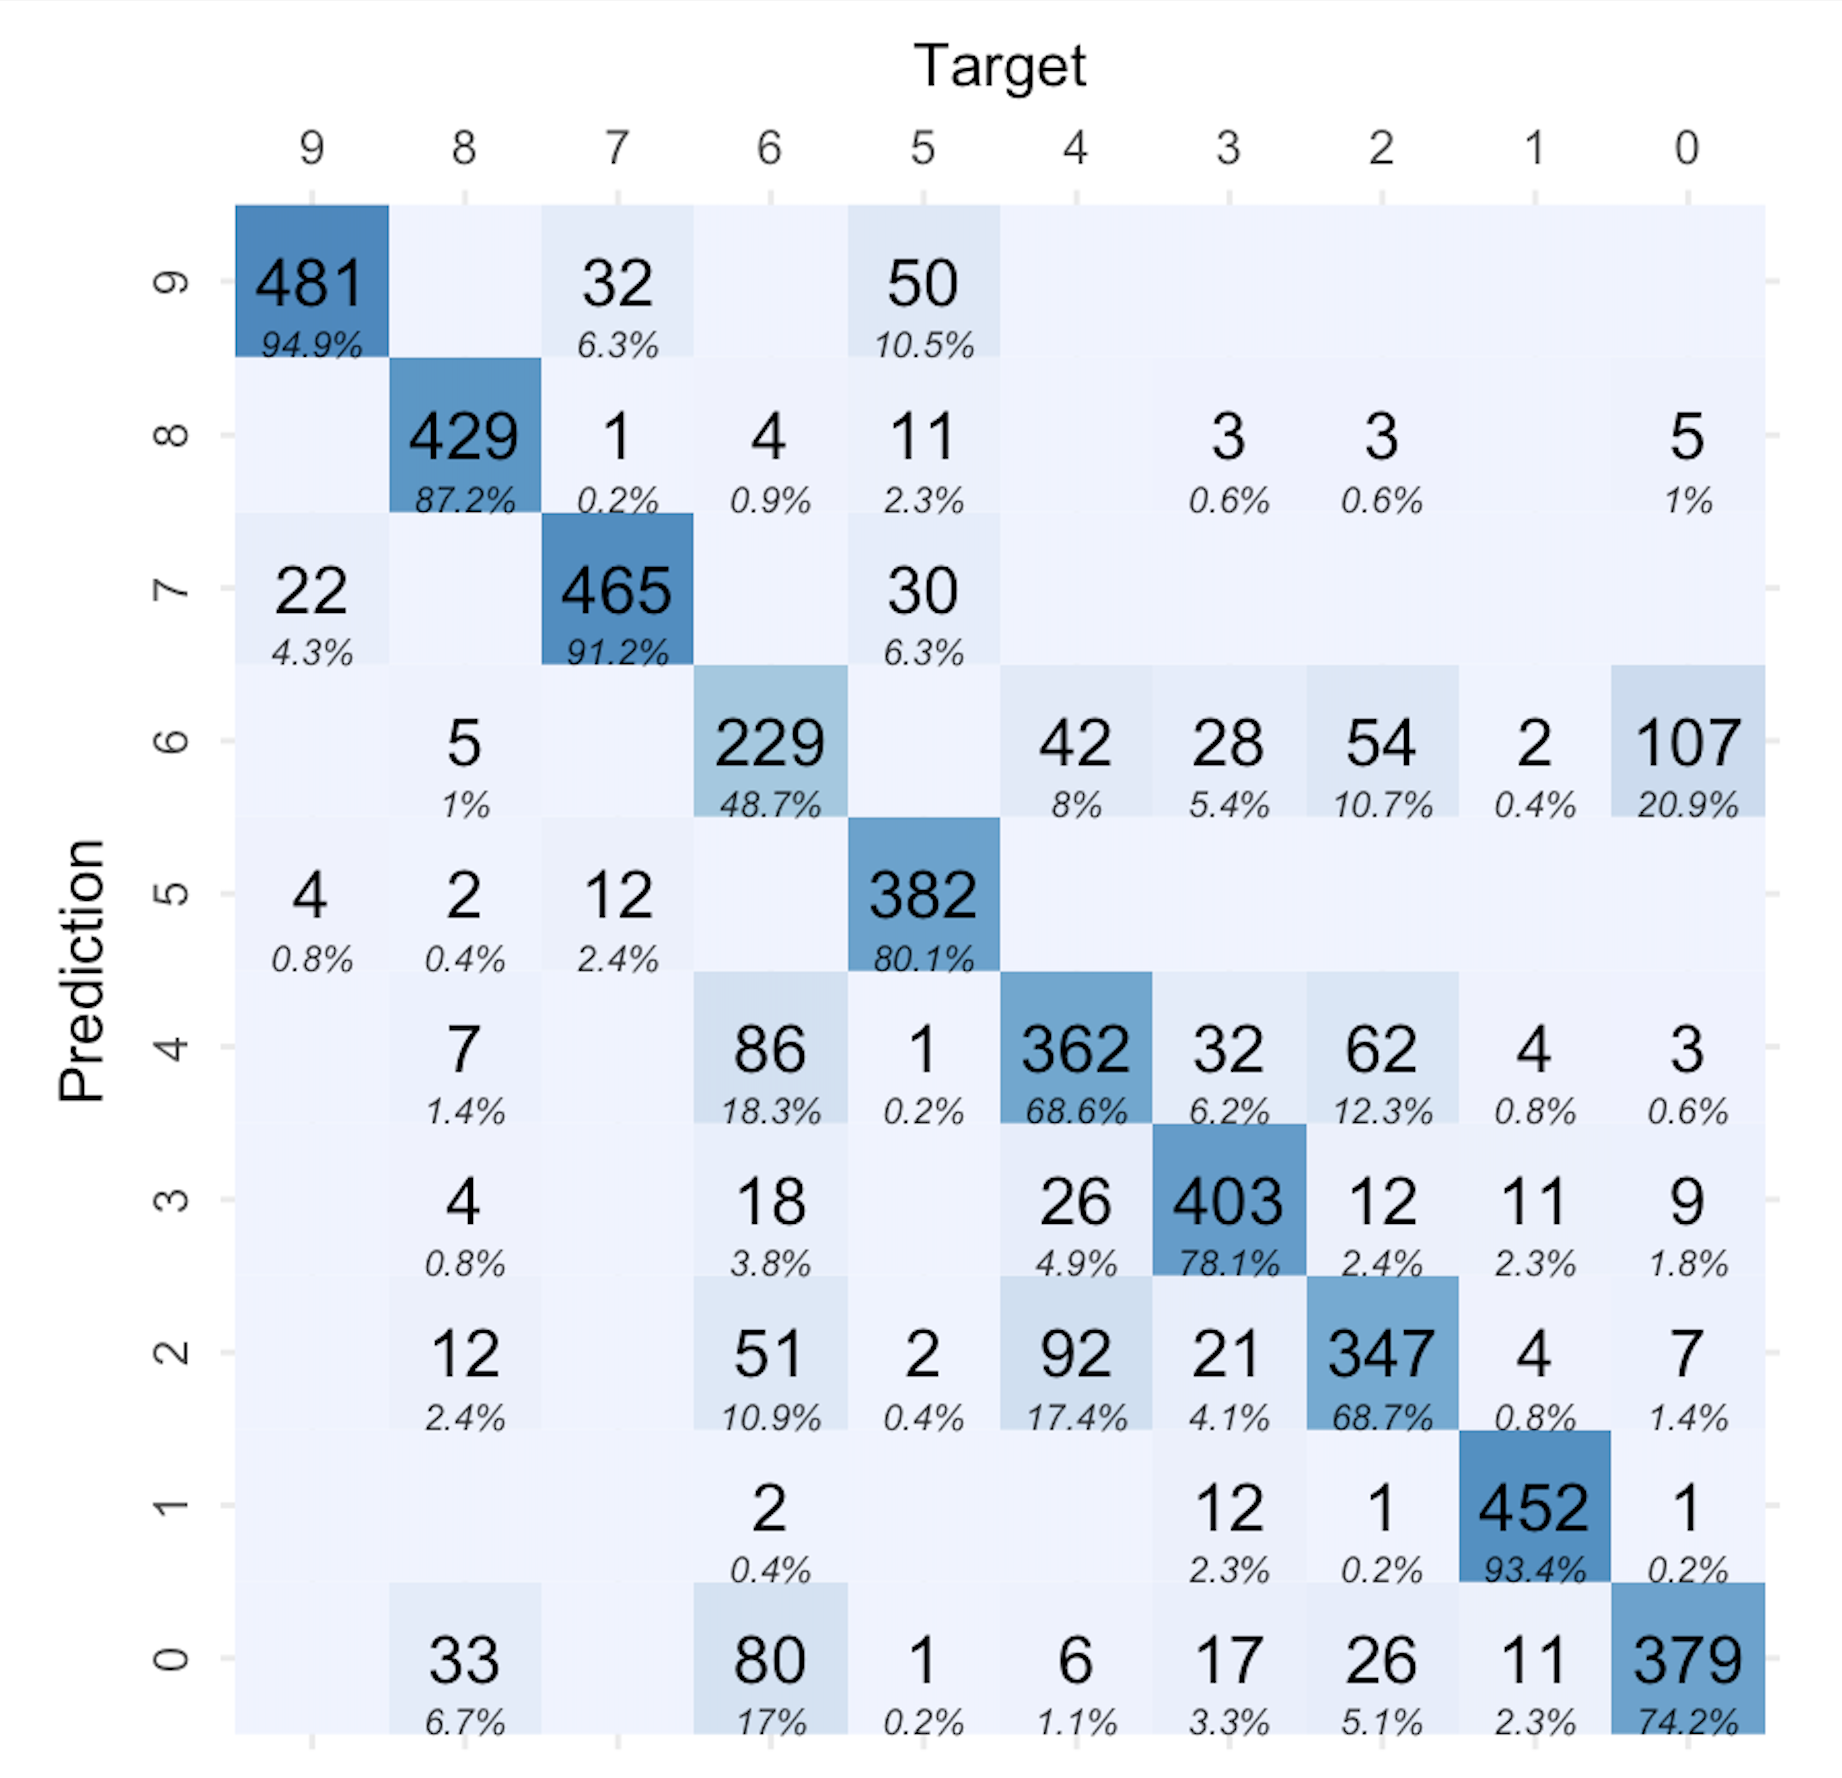
\includegraphics[width=0.36\textwidth]{figures/Fig10LeftConfMat.png}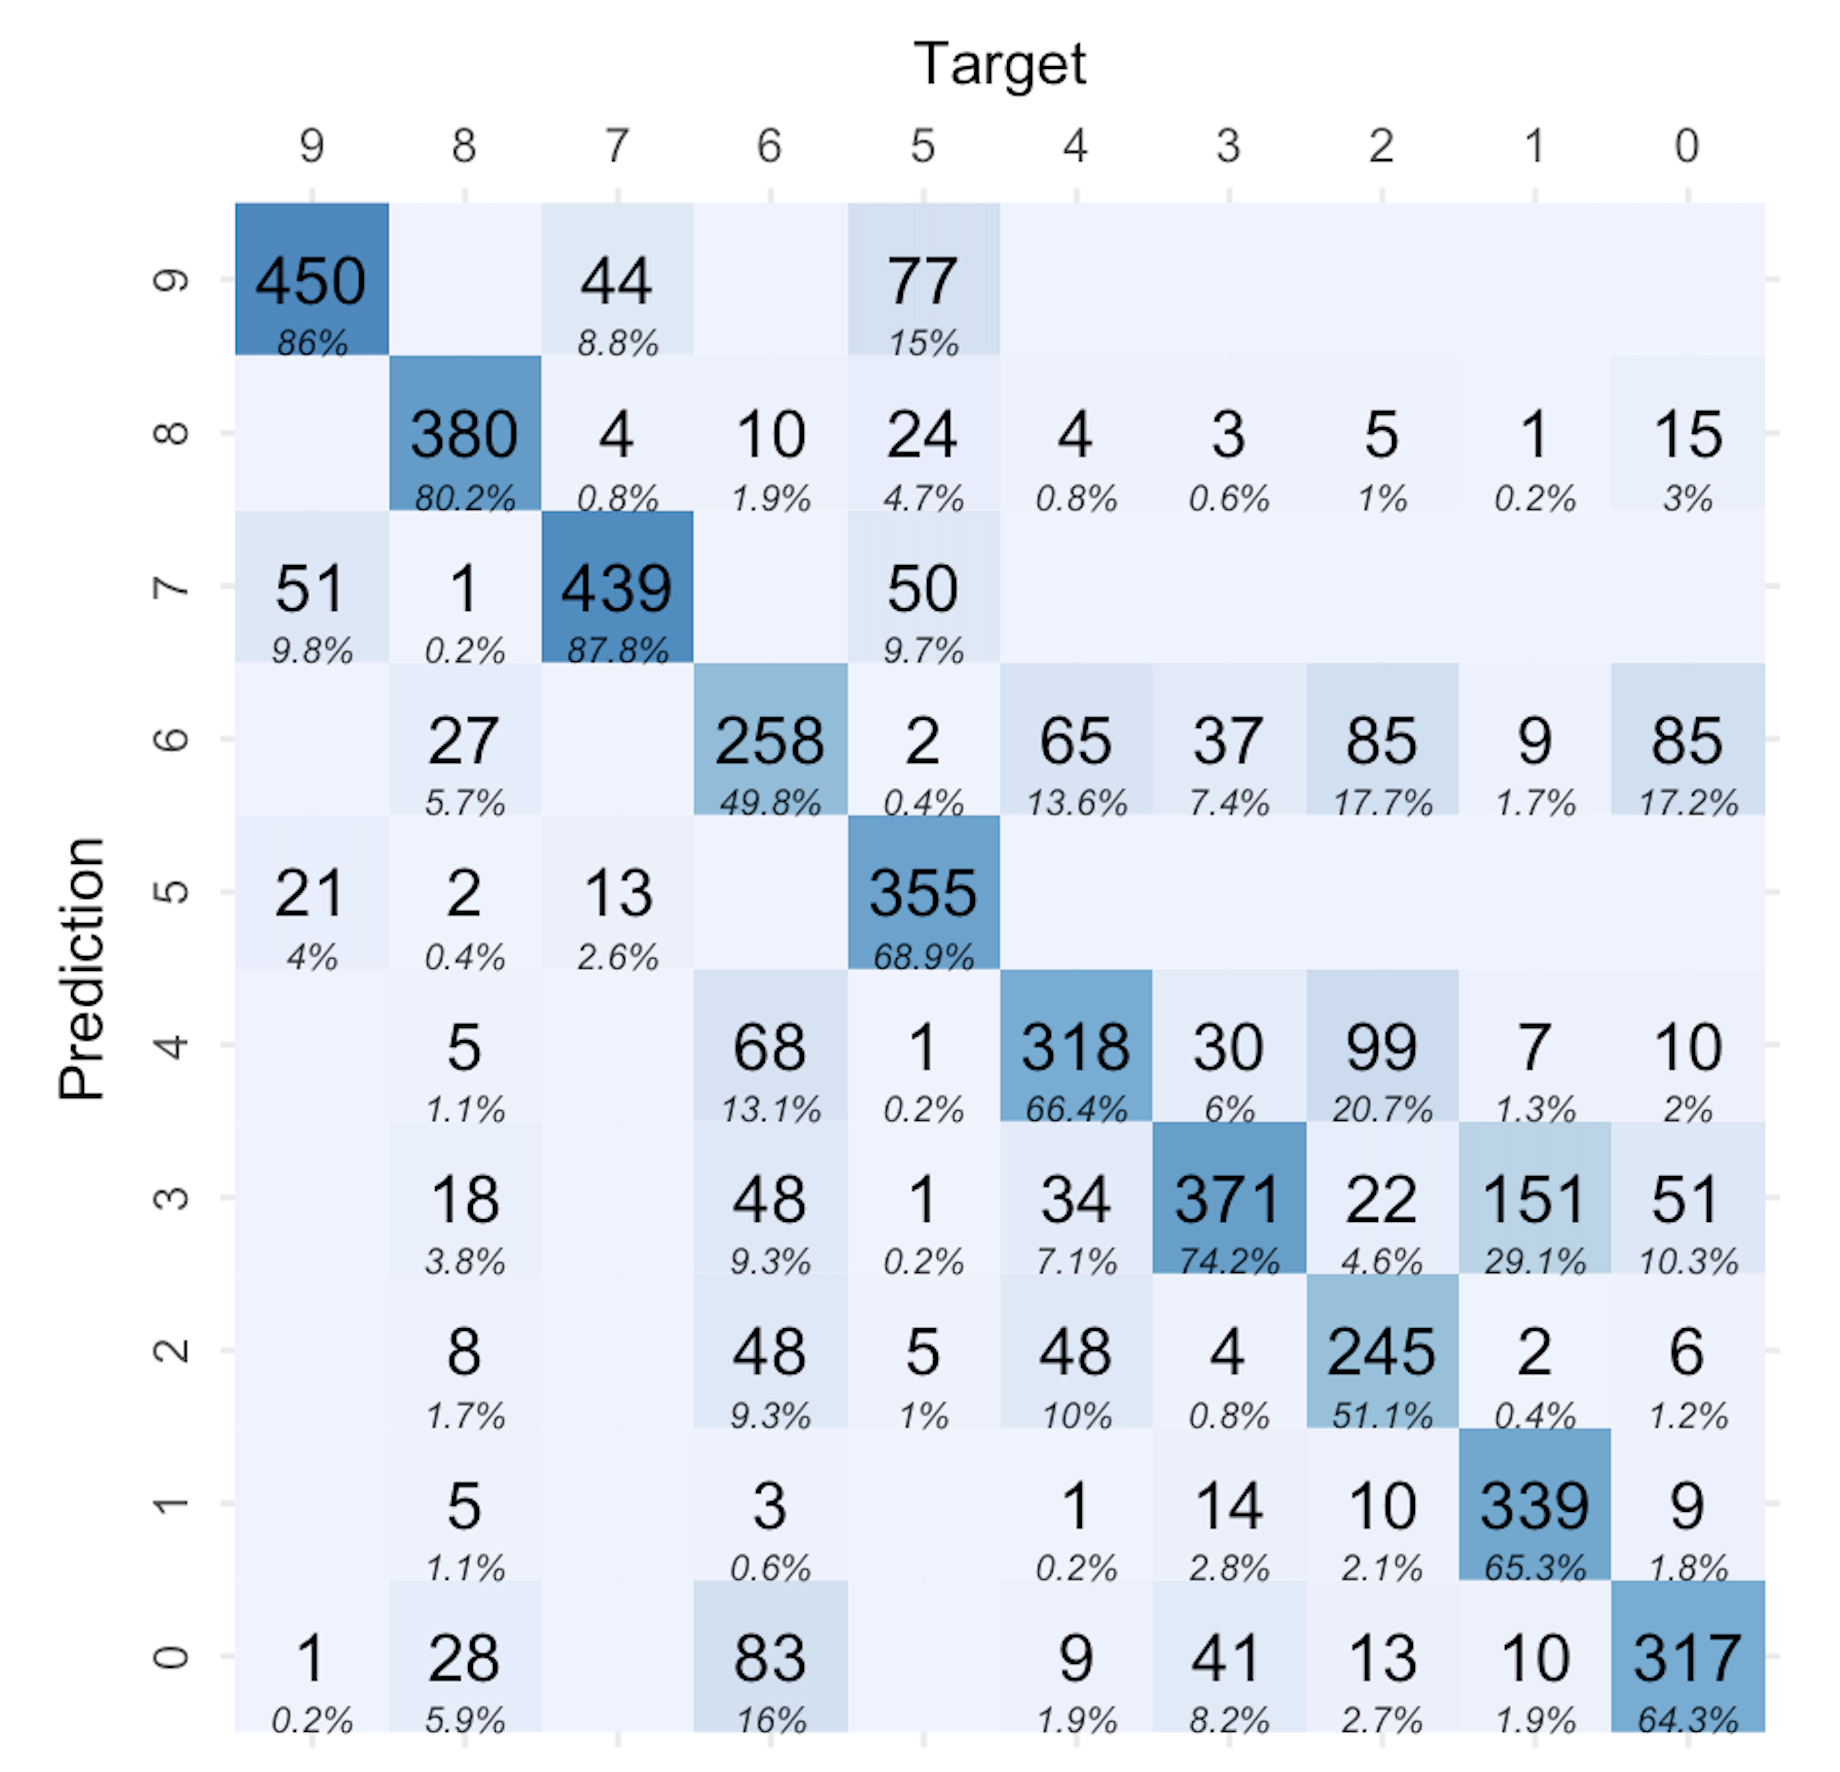
\includegraphics[width=0.36\textwidth]{figures/Fig10MiddleConfMat.png}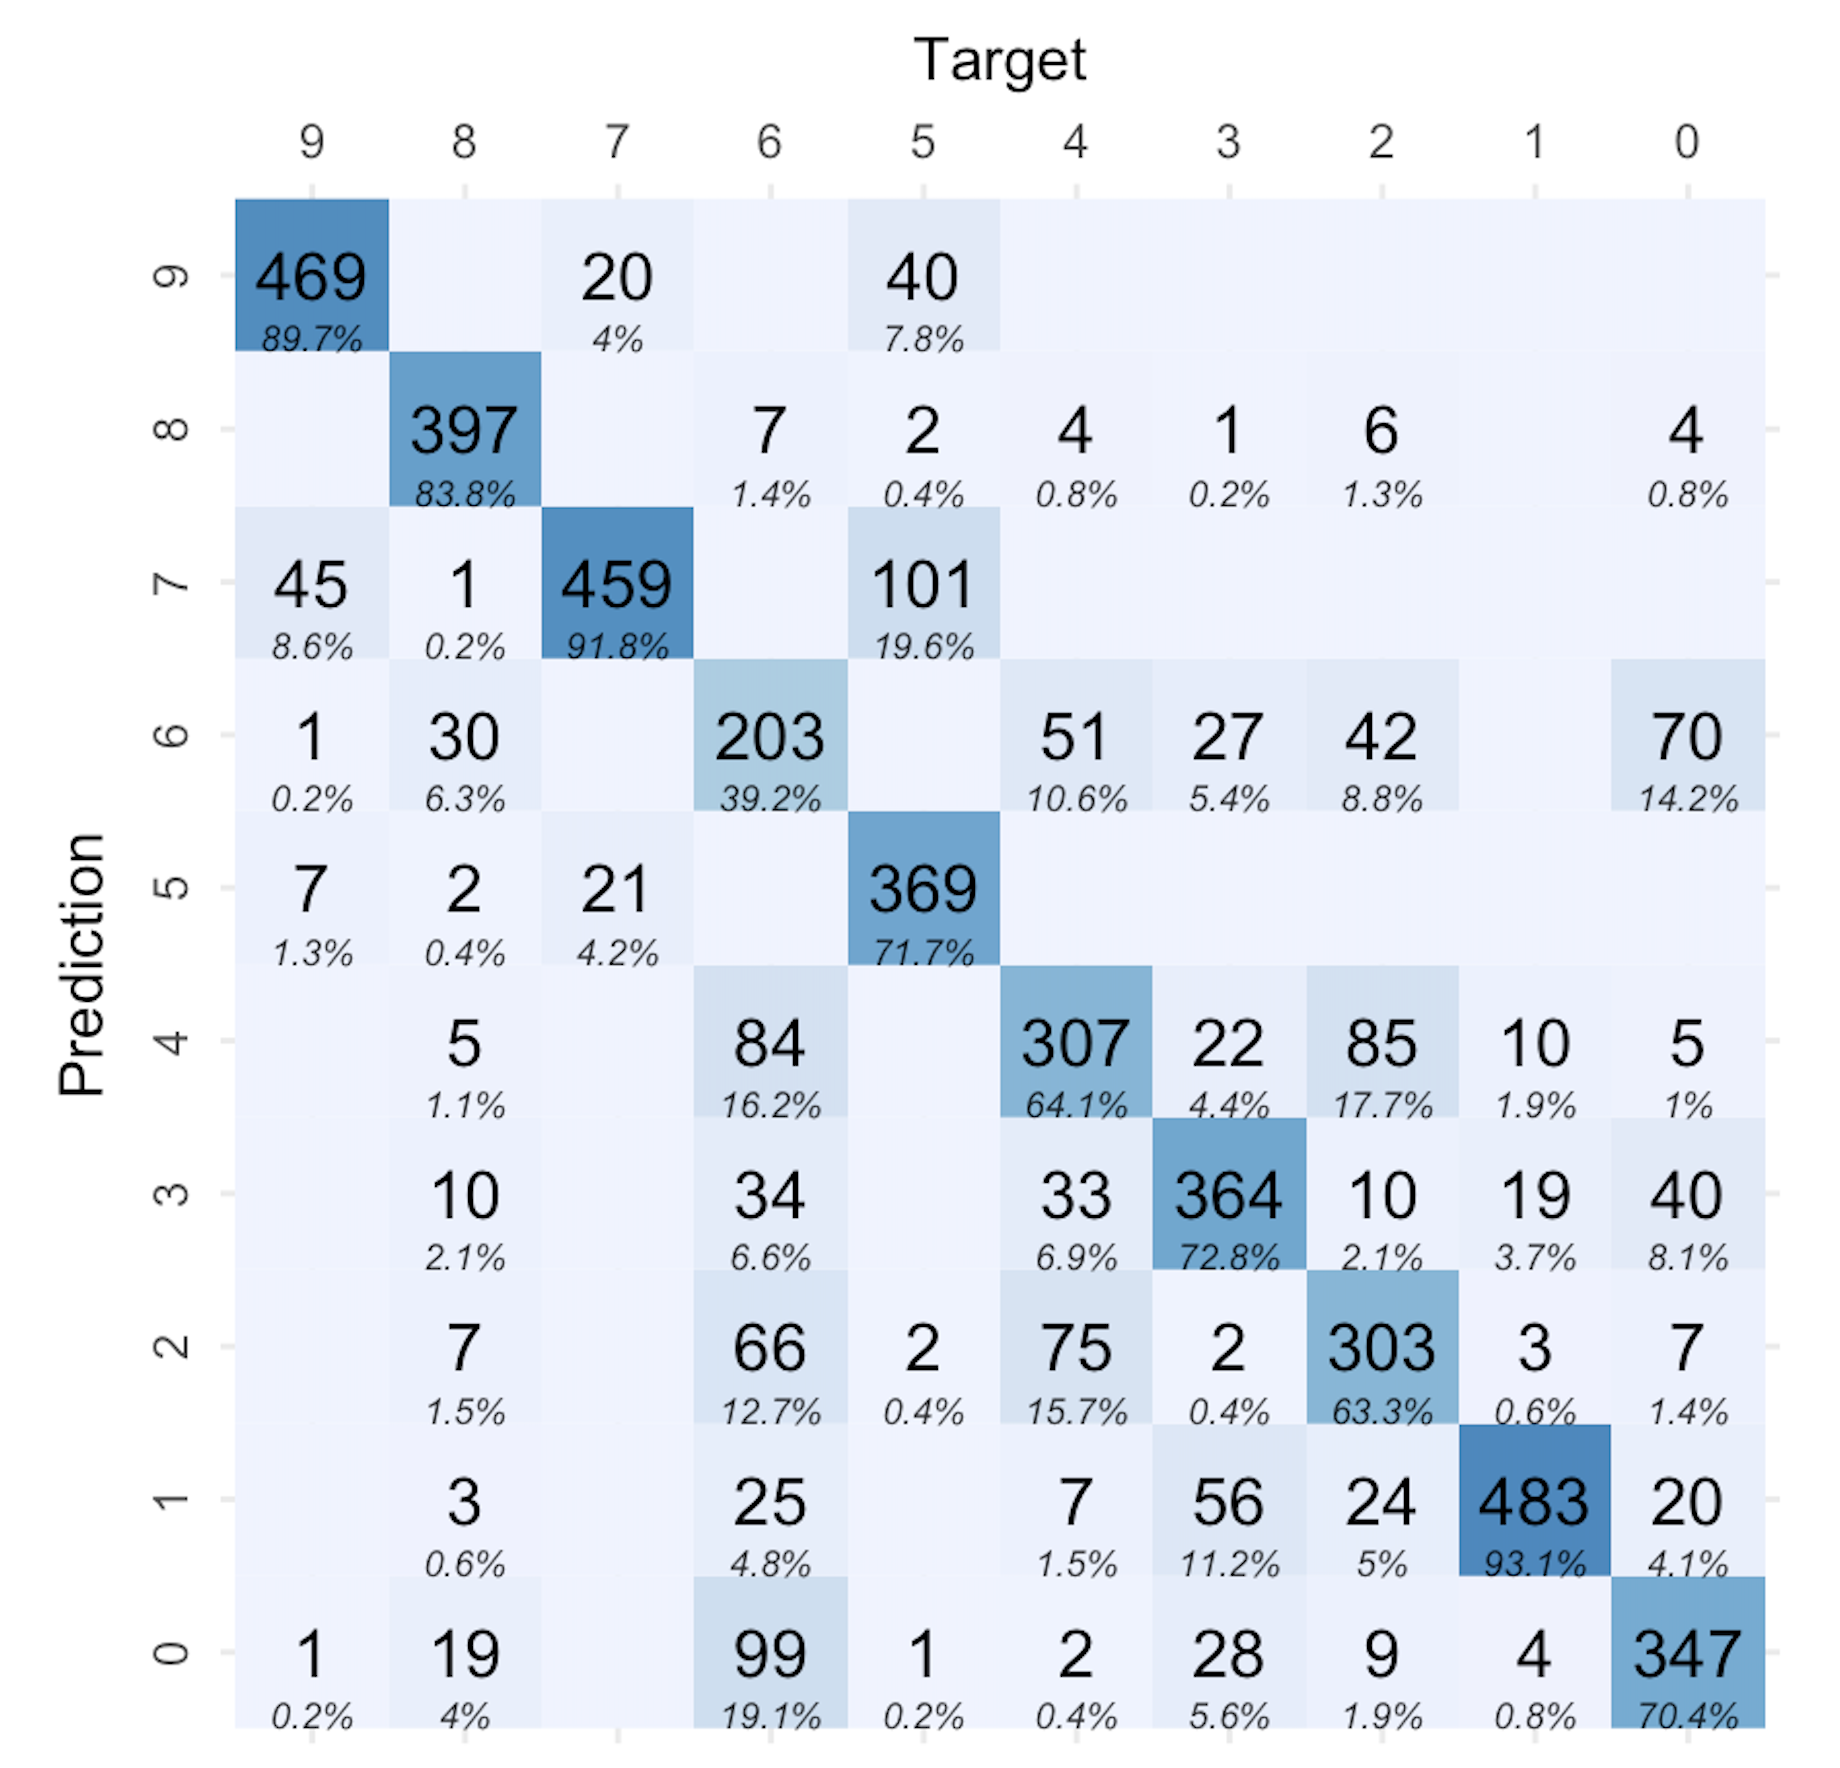
\includegraphics[width=0.36\textwidth]{figures/Fig10RightConfMat.png}
  \caption{Confusion matrix for S1, S2, and S3 from right to left.}\vspace{-.22cm}
  \label{CM}
  \end{figure}

The choice of these scenarios stems largely from our belief that the data targeted knot selection method leads to a more efficient dimension reduction, especially in the context of sparse data. As evidenced in Figure~\ref{HC}, the pixel distribution in the by-row data does not exhibit sparsity. This suggests that we might not see significant performance gains if we were to deploy the data based knot selection methodology on it.
However, the introduction of the Hilbert curve transformation imparts a noticeable sparsity in the data's curvature. 


As detailed above, we project the data into a subspace spanned by a number of eigenfunctions. For each scenario, we chose a number of eigenfunctions that achieved the highest accuracy on the validation data set. The validation phase of the analysis suggests that the optimal number of eigenvalues for S1, S2, and S3 are 15, 10, and 15, respectively. After the testing phase, we carry the classification problem described earlier across the three scenarios.
To evaluate the performance of our classification model, we define the following metrics
\begin{equation*}\footnotesize
        \text{Accuracy} = \frac{T_P + T_N}{T_P + T_N + F_P + F_N}, \ \ \ \  \text{Precision} = \frac{T_P}{T_P + F_P}, \ \ \ \  \text{Recall} = \frac{T_P}{T_P + F_N}, \ \ \ \ \text{F1} = 2 \, \frac{\text{Precision} \times \text{Recall}}{\text{Precision} + \text{Recall}},
        \end{equation*}
        where $T_P, T_N, F_P, F_N$ are true positives, true negatives, false positives and false negatives, respectively. 
Table \ref{3scenarios} presents the outcomes obtained from analyzing the classification problem within the three suggested scenarios.



\begin{table}[h]
\centering
\caption{\footnotesize Accuracy, Precision, Recall and F1 Score of the classification problem in each scenario.}
\centering
 \resizebox{0.7\columnwidth}{!}{
  \tiny
 \begin{tabular}{c c c c } \toprule
  & \bf Scenario 1 & \bf Scenario 2 & \bf Scenario 3\\ \hline 
\bf Accuracy&  $78.6\%$ & $69.44\%$ & $73.6\%$ \\ 
\bf Precision&  $79.22\%$ & $71.3\%$ & $74.1 \%$ \\
\bf Recall&  $78.5\%$ & $69.4\%$ & $73.9\%$ \\
\bf F1&  $78.74\%$ & $69.8\%$ & $73.6\%$ \\
\bottomrule
\end{tabular}
}
\label{3scenarios}
\end{table}
\vspace{-.22cm}
The results from the first scenario (S1) clearly demonstrate its superior performance, affirming our proposition. To further understand the algorithm's misclassifications, we provide the confusion matrix for each scenario in Figure \ref{CM}. The confusion matrix illustrates the comparison between the true labels and the predicted labels of the test dataset. The confusion matrices show the uncertainty mostly between the classes 0,2,4,6 in the fashion image dataset, as discussed in the previous section . This makes sense because t-shirts, pullovers, coats, and shirts look similar and might be confusing.
 
 In the absence of the Hilbert curve transformation, it is observed that the classification performance of the data-driven knot selection approach alone is the least accurate among the three scenarios. This is consistent with expectations given that the data exhibits a dense and non-sparse format with highly repetitive patterns.
 %the uniform pattern exhibited by the data. 
 The equidistant knot selection classification strategy shows a modest increment in the accuracy results. However, the application of data-driven knot selection on the transformed data significantly improves the accuracy of the results. It is important to note that our aim is not to outperform or compete with state-of-the-art machine learning and deep learning methodologies in image classification. 
 %Although our method may not achieve the highest levels of accuracy, it does attain a reasonably close accuracy rate of approximately $80\% $, comparable to some basic three-layer and four-layer neural networks. Our method, while not the most accurate, does achieve an accuracy level close to $80\% $, comparable to some simplistic neural networks such as decision tree classifiers, MLP Classifiers. For more benchmarking machine learning algorithms classifiers on Fashoin MNIST data set see \cite{xiao2017fashion}. 
 Although our method may not achieve the the optimal accuracy levels that can be seen in the convolution neural network approach, it does reach a commendable accuracy rate of approximately $80\%$. This is comparable to simpler neural networks, such as decision tree classifiers and MLP classifiers. For further benchmarking of machine learning algorithm classifiers on the Fashion MNIST dataset, see \citep{xiao2017fashion}. The implementation of the Hilbert curve transformation highlights the effectiveness of the data-driven method for representing data in a functional format, resulting a noticeable increase in accuracy by $5-6\%$. This enhancement is attributed to the efficient representation of locality features in the data through the chosen basis, ensuring the preservation of space curvature.
 %This is achieved through the efficient representation of locality features in the data via the selected basis, preserving the space curvature. 
 
There are two notable observations to consider. First, the data-driven knot selection method demonstrates superior performance compared to the traditional equidistance method, especially when handling sparse data that exhibits distinct spatial dependencies. This difference in performance can be observed by comparing the class-wise accuracy between S1, S2, and S3. Second, leveraging the 2D characteristics of the images has a positive impact on the performance of Functional Principal Component Analysis (FPCA) when combined with the data-driven knot selection method. A transformation such as the Hilbert curve, can reveal the two-dimensional characteristics of the original image by preserving the locality relationships among the pixels. More precisely, in the flattened one-dimensional vector, consecutive elements (pixels) were likely neighbors in the original two-dimensional space. It also creates a sparser representation of the image, which makes it more amenable to our method. Therefore, when we apply our FPCA data-driven analysis techniques to this one-dimensional vector, these techniques approximately analyze the local neighborhoods of the original two-dimensional image. This enhancement suggests, as expected, that considering the 2D structure of the images contributes to improved results and should be further investigated.

\vspace{-.13cm}
\section{Summary}
\vspace{-.22cm}
We have presented tools from the \pkg{Splinets}-package that facilitate an efficient analysis of functional data. The benefits using the orthogonal basis implemented in the package are illustrated both by a simple example of the FPCA performed on the classical wine data set and by a more advanced workflow for classification of functional data. 
This workflow is designed to enhance the efficiency of dimension reduction while retaining functional dependencies in the data's characterizing features, which may not necessarily be local. 
The workflow was benchmarked on the Fashion MNIST data set. 
The findings from this example emphasize the pivotal importance of the data's two-dimensional nature in the functional principal component analysis approach. 
%underline the central significance of the data's two-dimensional character in the functional principal component analysis approach.
The Hilbert curve proved to be the most efficient and it is partially due to its capacity of capturing dependencies beyond one dimension. 
These observations suggest that adopting the method further toward two-dimensional analysis, for example, by considering gradient images or, even better, two-dimensional FPCA may lead to significant gains in the efficiencies.



\vspace{-.1cm}


\bibliography{RJreferences.bib}

\address{%
Rani Basna\\
Department of Clinical Sciences\\%
Lund University\\ Sweden\\ \url{Rani.Basna@med.lu.se}\\
%
%
%
%
}

\address{%
Hiba Nassar\\
Cognitive Systems, Department of Applied Mathematics and Computer
Science\\%
Technical University of Denmark\\ Denmark\\ \url{hibna@dtu.dk}\\
%
%
%
%
}

\address{%
Krzysztof Podgórski\\
Department of Statistics\\%
Lund University\\ Sweden\\ \url{Krzysztof.Podgorski@stat.lu.se}\\
%
%
%
%
}
